\documentclass[12pt,a4paper,titlepage]{article}

\usepackage{xcolor}
\usepackage{minted}
\usepackage{caption}
\usepackage{tabularx}
\usepackage{graphicx}
\usepackage{titlesec}
\usepackage{indentfirst}
\usepackage[portuguese]{babel}
\usepackage[colorlinks=true,allcolors=black]{hyperref}

\graphicspath{{./img/}{./../../../}{./img/tb_verilog}}
\newcommand{\sectionbreak}{\clearpage}
\setminted
{
    linenos,
    frame=single,
    breaklines
}

\title
{
Arquitetura de Computadores II\\
Lista X\\
[1.5em]
\centering

\includegraphics[scale=0.8]{puc.png}
}

\author{Fernando de Lima Gonçalves}
\date{Belo Horizonte\\10/2026}

\begin{document}
\maketitle
\tableofcontents

% Blocos de Codigos
% Verilog
\section{Blocos RISC-V: Verilog}
\subsection{Instruction Fetch}
\subsubsection{Memória de Instrução}
\inputminted{v}{./code/verilog/instruction_memory.v}

\clearpage\subsubsection{Módulo de Busca}
\inputminted{v}{./code/verilog/if_stage.v}

\clearpage\subsection{Instruction Decode (ID)}
\subsubsection{Banco de Registradores}
\inputminted{v}{./code/verilog/register_file.v}

\clearpage\subsubsection{Gerador de Imediatos}
\inputminted{v}{./code/verilog/imm_gen.v}

\clearpage\subsubsection{Módulo de Decodificação}
\inputminted{v}{./code/verilog/id_stage.v}

\clearpage\subsection{Control Unit}
\subsubsection{Unidade de Controle}
\inputminted{v}{./code/verilog/control_unit.v}

\clearpage\subsection{Execution}
\inputminted{v}{./code/verilog/ex_stage.v}

\subsection{Memory Unit}
\inputminted{v}{./code/verilog/mem_stage.v}

\subsection{Write Back}
\inputminted{v}{./code/verilog/wb_stage.v}

\clearpage
\subsection{Bloco Top-Level: RISC-V}
\inputminted{v}{./code/verilog/riscv_top.v}

% Java
\section{Blocos RISC-V: Java}
Os blocos de código \texttt{Java} foram traduzidos da linguagem \texttt{verilog} 
via \texttt{LLM GPT-6} em esforço médio.

\subsection{Instruction Fetch}
\subsubsection{Memória de Instrução}
\inputminted{java}{./code/java/instruction_memory.java}

\clearpage\subsubsection{Módulo de Busca}
\inputminted{java}{./code/java/if_stage.java}

\clearpage
\subsection{Instruction Decode (ID)}
\subsubsection{Banco de Registradores}
\inputminted{java}{./code/java/register_file.java}

\clearpage\subsubsection{Gerador de Imediatos}
\inputminted{java}{./code/java/imm_gen.java}

\clearpage\subsubsection{Módulo de Decodificação}
\inputminted{java}{./code/java/id_stage.java}

\clearpage
\subsection{Control Unit}
\inputminted{java}{./code/java/control_unit.java}

\clearpage\subsection{Execution}
\inputminted[fontsize=\small]{java}{./code/java/ex_stage.java}

\subsection{Memory Unit}
\inputminted{java}{./code/java/mem_stage.java}

\subsection{Write Back}
\inputminted{java}{./code/java/wb_stage.java}

\clearpage
\subsection{Bloco Top-Level: RISC-V}
\inputminted[fontsize=\small]{java}{./code/java/riscv_top.java}

\section{Testbench}
\subsection{Descrição}
\begin{itemize}
    \item \textbf{instruction\_memory:}
    O teste percorre os endereços 0, 4, 8 e 9, verificando a leitura das instruções ADD, LW e SW armazenadas na ROM, além do alinhamento por palavra.

    \item \textbf{if\_stage:}
    O teste verifica o incremento do PC de quatro em quatro, o desvio para o endereço 16 por meio de \texttt{pc\_src} e 
    seu retorno a zero após o sinal de reset.

    \item \textbf{register\_file:}
    O teste escreve os valores 10 e 20 em \texttt{x1} e \texttt{x2}, verifica a leitura desses registradores e confirma que \texttt{x0} não 
    pode ser modificado e que a escrita pode ser desabilitada.

    \item \textbf{imm\_gen:}
    O teste utiliza instruções LW, SW e BEQ com imediatos positivos e negativos, verificando a extração e a extensão de sinal, além do imediato zero para ADD.

    \item \textbf{id\_stage:}
    O teste inicializa \texttt{x1} a \texttt{x4} com valores de 10 a 40 e decodifica instruções ADD, SUB, LW, SW e BEQ, verificando os 
    campos da instrução, os operandos e o imediato.

    \item \textbf{control\_unit:}
    O teste alterna \texttt{opcode}, \texttt{funct3} e \texttt{funct7\_5} entre ADD, SUB, AND, OR, LW, SW e BEQ, verificando os 
    sinais de controle da ALU, memória e registradores.

    \item \textbf{ex\_stage:}
    O teste realiza ADD, SUB, AND e OR com operandos 10 e 5, além de testar a soma com imediato, o sinal \texttt{zero} e o cálculo do 
    destino de desvio para PC = 100.

    \item \textbf{mem\_stage:}
    O teste grava 100 e 200 nos endereços 0 e 4, verifica suas leituras e confirma que os sinais \texttt{mem\_read} e \texttt{mem\_write} 
    controlam as operações de memória.

    \item \textbf{wb\_stage:}
    O teste alterna \texttt{mem\_to\_reg} entre 0 e 1, verificando a seleção dos resultados da ALU (15, 25 e 50) ou dos 
    dados da memória (100 e 200) para escrita.

    \item \textbf{riscv\_top:}
    O teste executa as três instruções integradas ADD, LW e SW, verificando a soma de \texttt{x1 = 4} e \texttt{x2 = 8}, a leitura do valor 99 da memória 
    e seu armazenamento em outro endereço.
\end{itemize}

\subsection{Códigos}
\subsubsection{Memória de Instrução}
\inputminted{v}{./code/verilog/test/tb_instruction_memory.v}

\clearpage\subsubsection{Módulo de Busca}
\inputminted{v}{./code/verilog/test/tb_if_stage.v}

\clearpage\subsubsection{Banco de Registradores}
\inputminted{v}{./code/verilog/test/tb_register_file.v}

\clearpage\subsubsection{Gerador de Imediatos}
\inputminted{v}{./code/verilog/test/tb_imm_gen.v}

\clearpage\subsubsection{Módulo de Decodificação}
\inputminted{v}{./code/verilog/test/tb_id_stage.v}

\clearpage\subsubsection{Unidade de Controle}
\inputminted{v}{./code/verilog/test/tb_control_unit.v}

\clearpage\subsubsection{Execution}
\inputminted{v}{./code/verilog/test/tb_ex_stage.v}

\clearpage\subsubsection{Memory Unit}
\inputminted{v}{./code/verilog/test/tb_mem_stage.v}

\clearpage\subsubsection{Write Back}
\inputminted{v}{./code/verilog/test/tb_wb_stage.v}

\clearpage\subsubsection{Bloco Top-Level: RISC-V}
\inputminted{v}{./code/verilog/test/tb_riscv_top.v}

\clearpage
\section{Simulação: TP Lab}
Todos os testes e formato de ondas foram obtidos por meio da aplicação \textit{TPLab}.

\subsection{Memória de Instrução}
\begin{figure}[h]
    \centering
    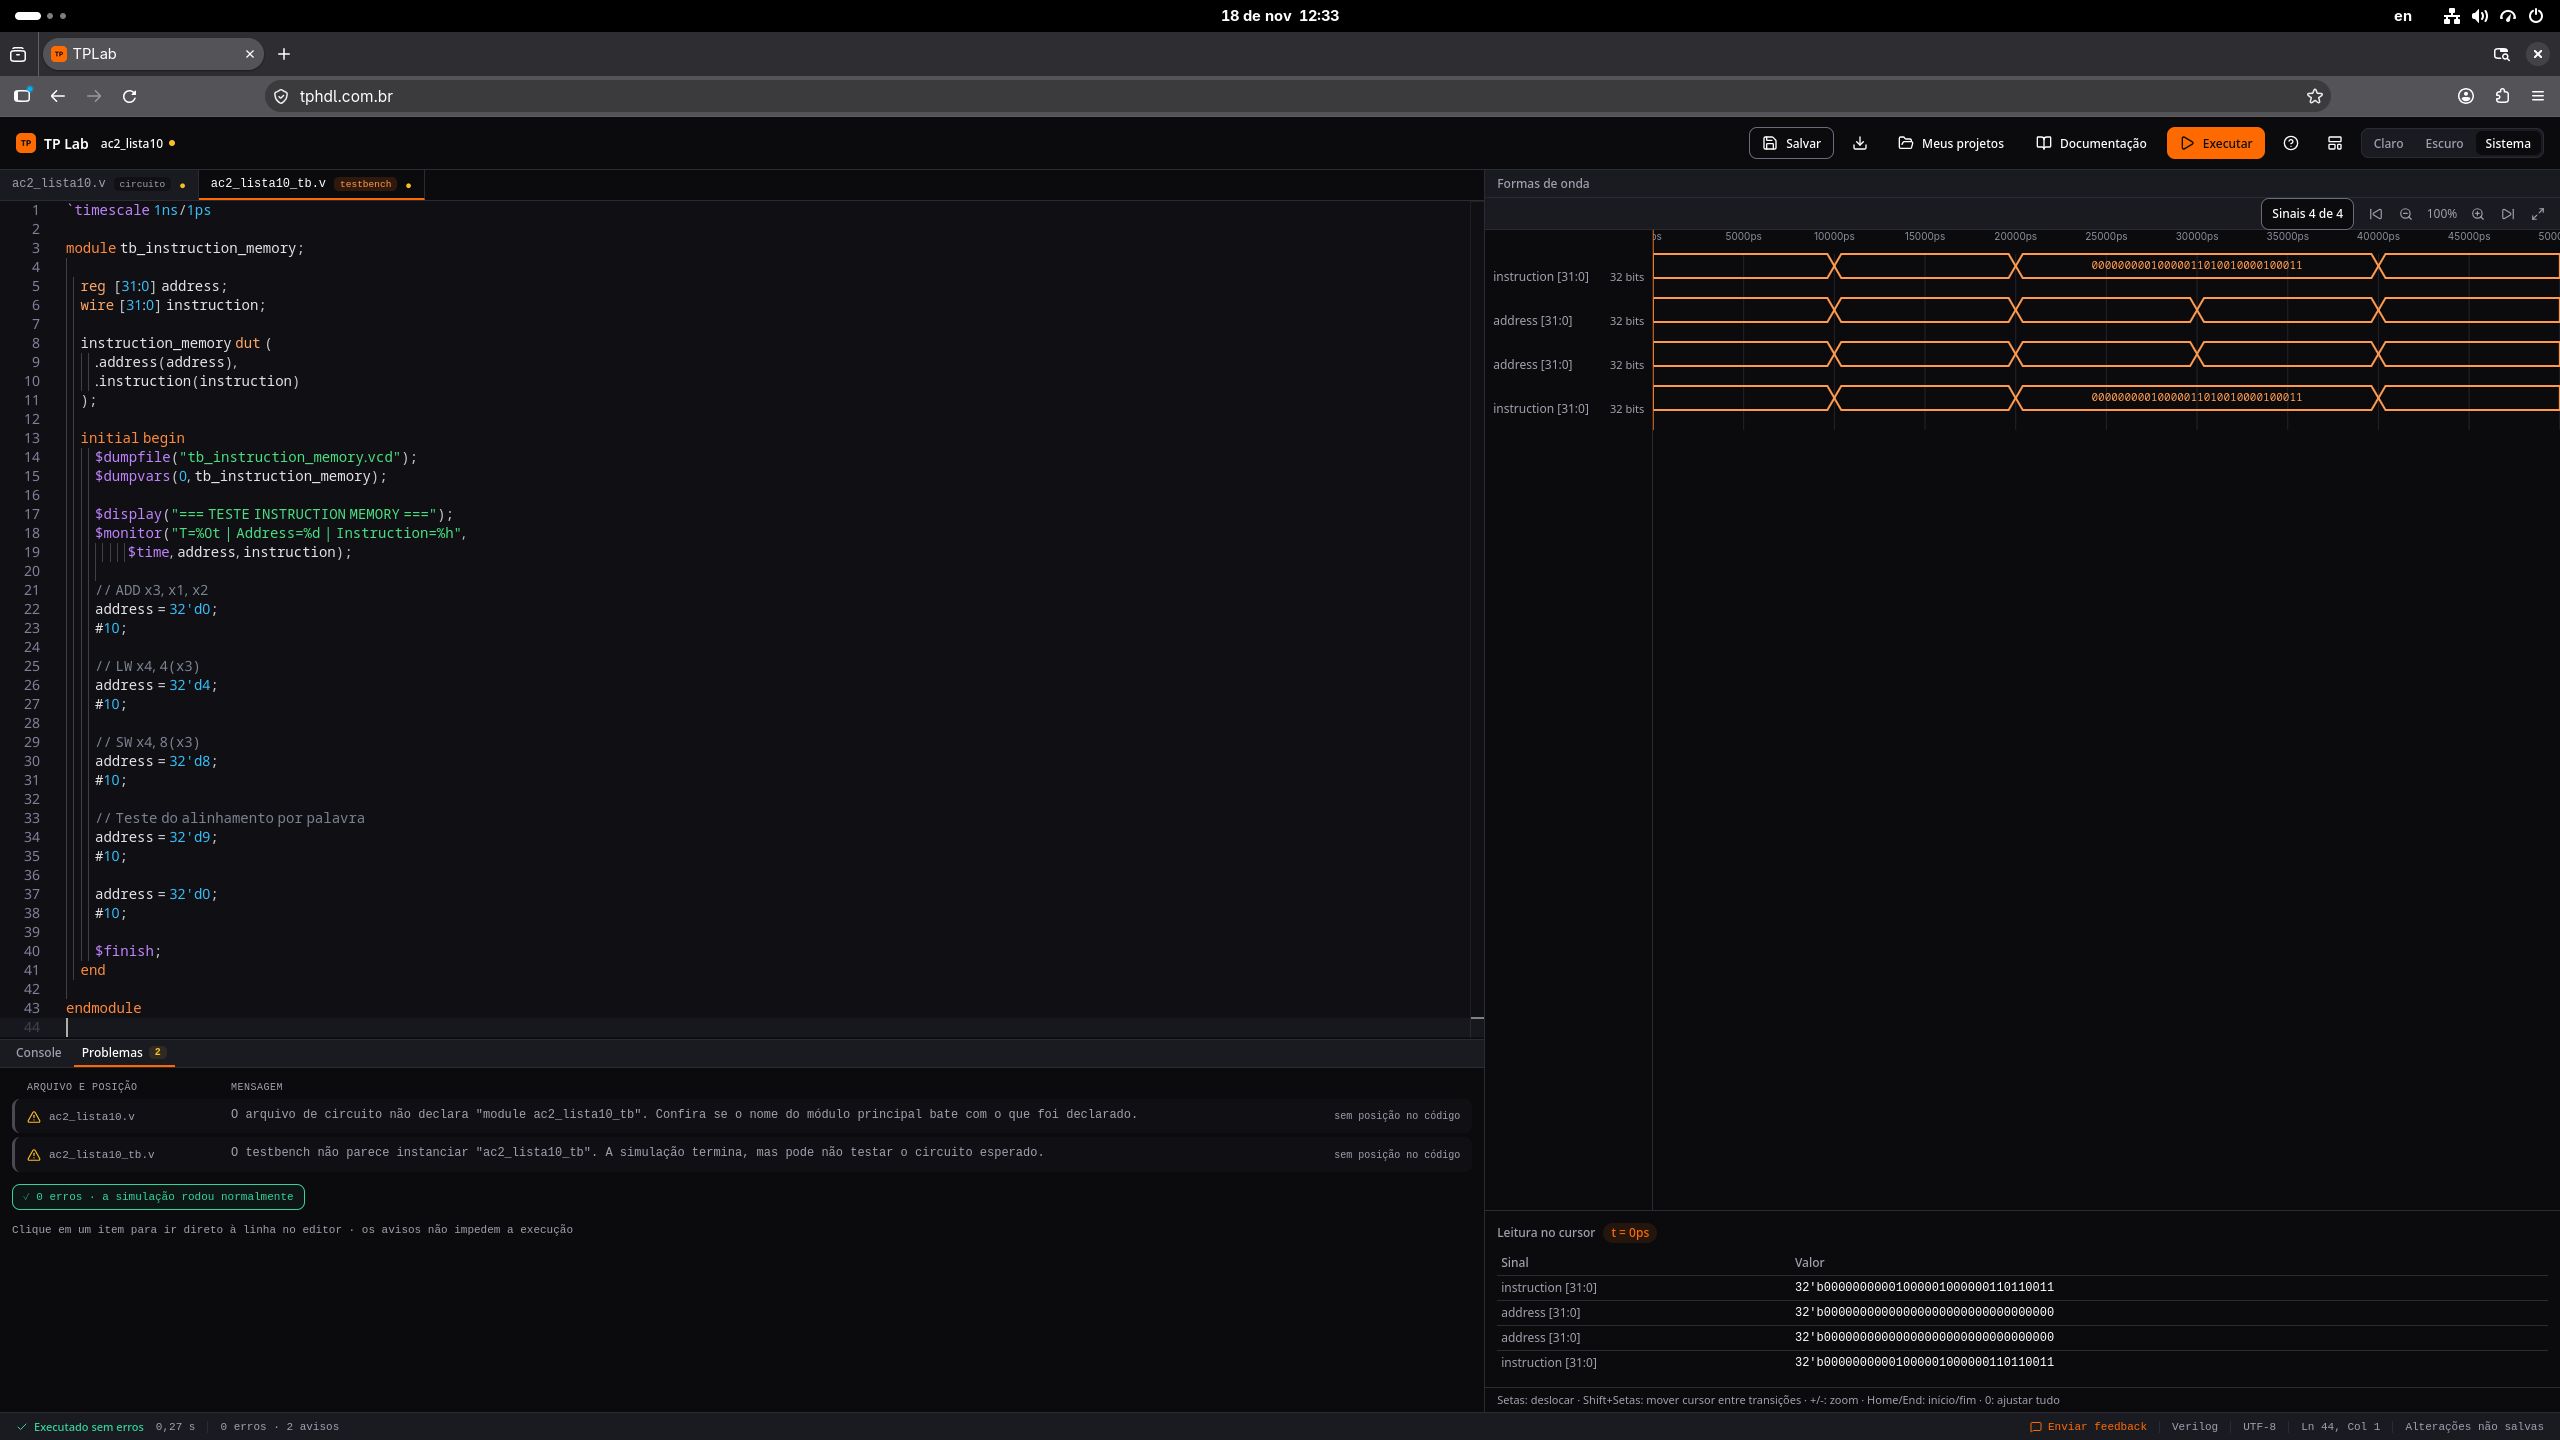
\includegraphics[scale=0.15]{tb_instruction_memory}
\end{figure}

\clearpage\subsection{Módulo de Busca}
\begin{figure}[h]
    \centering
    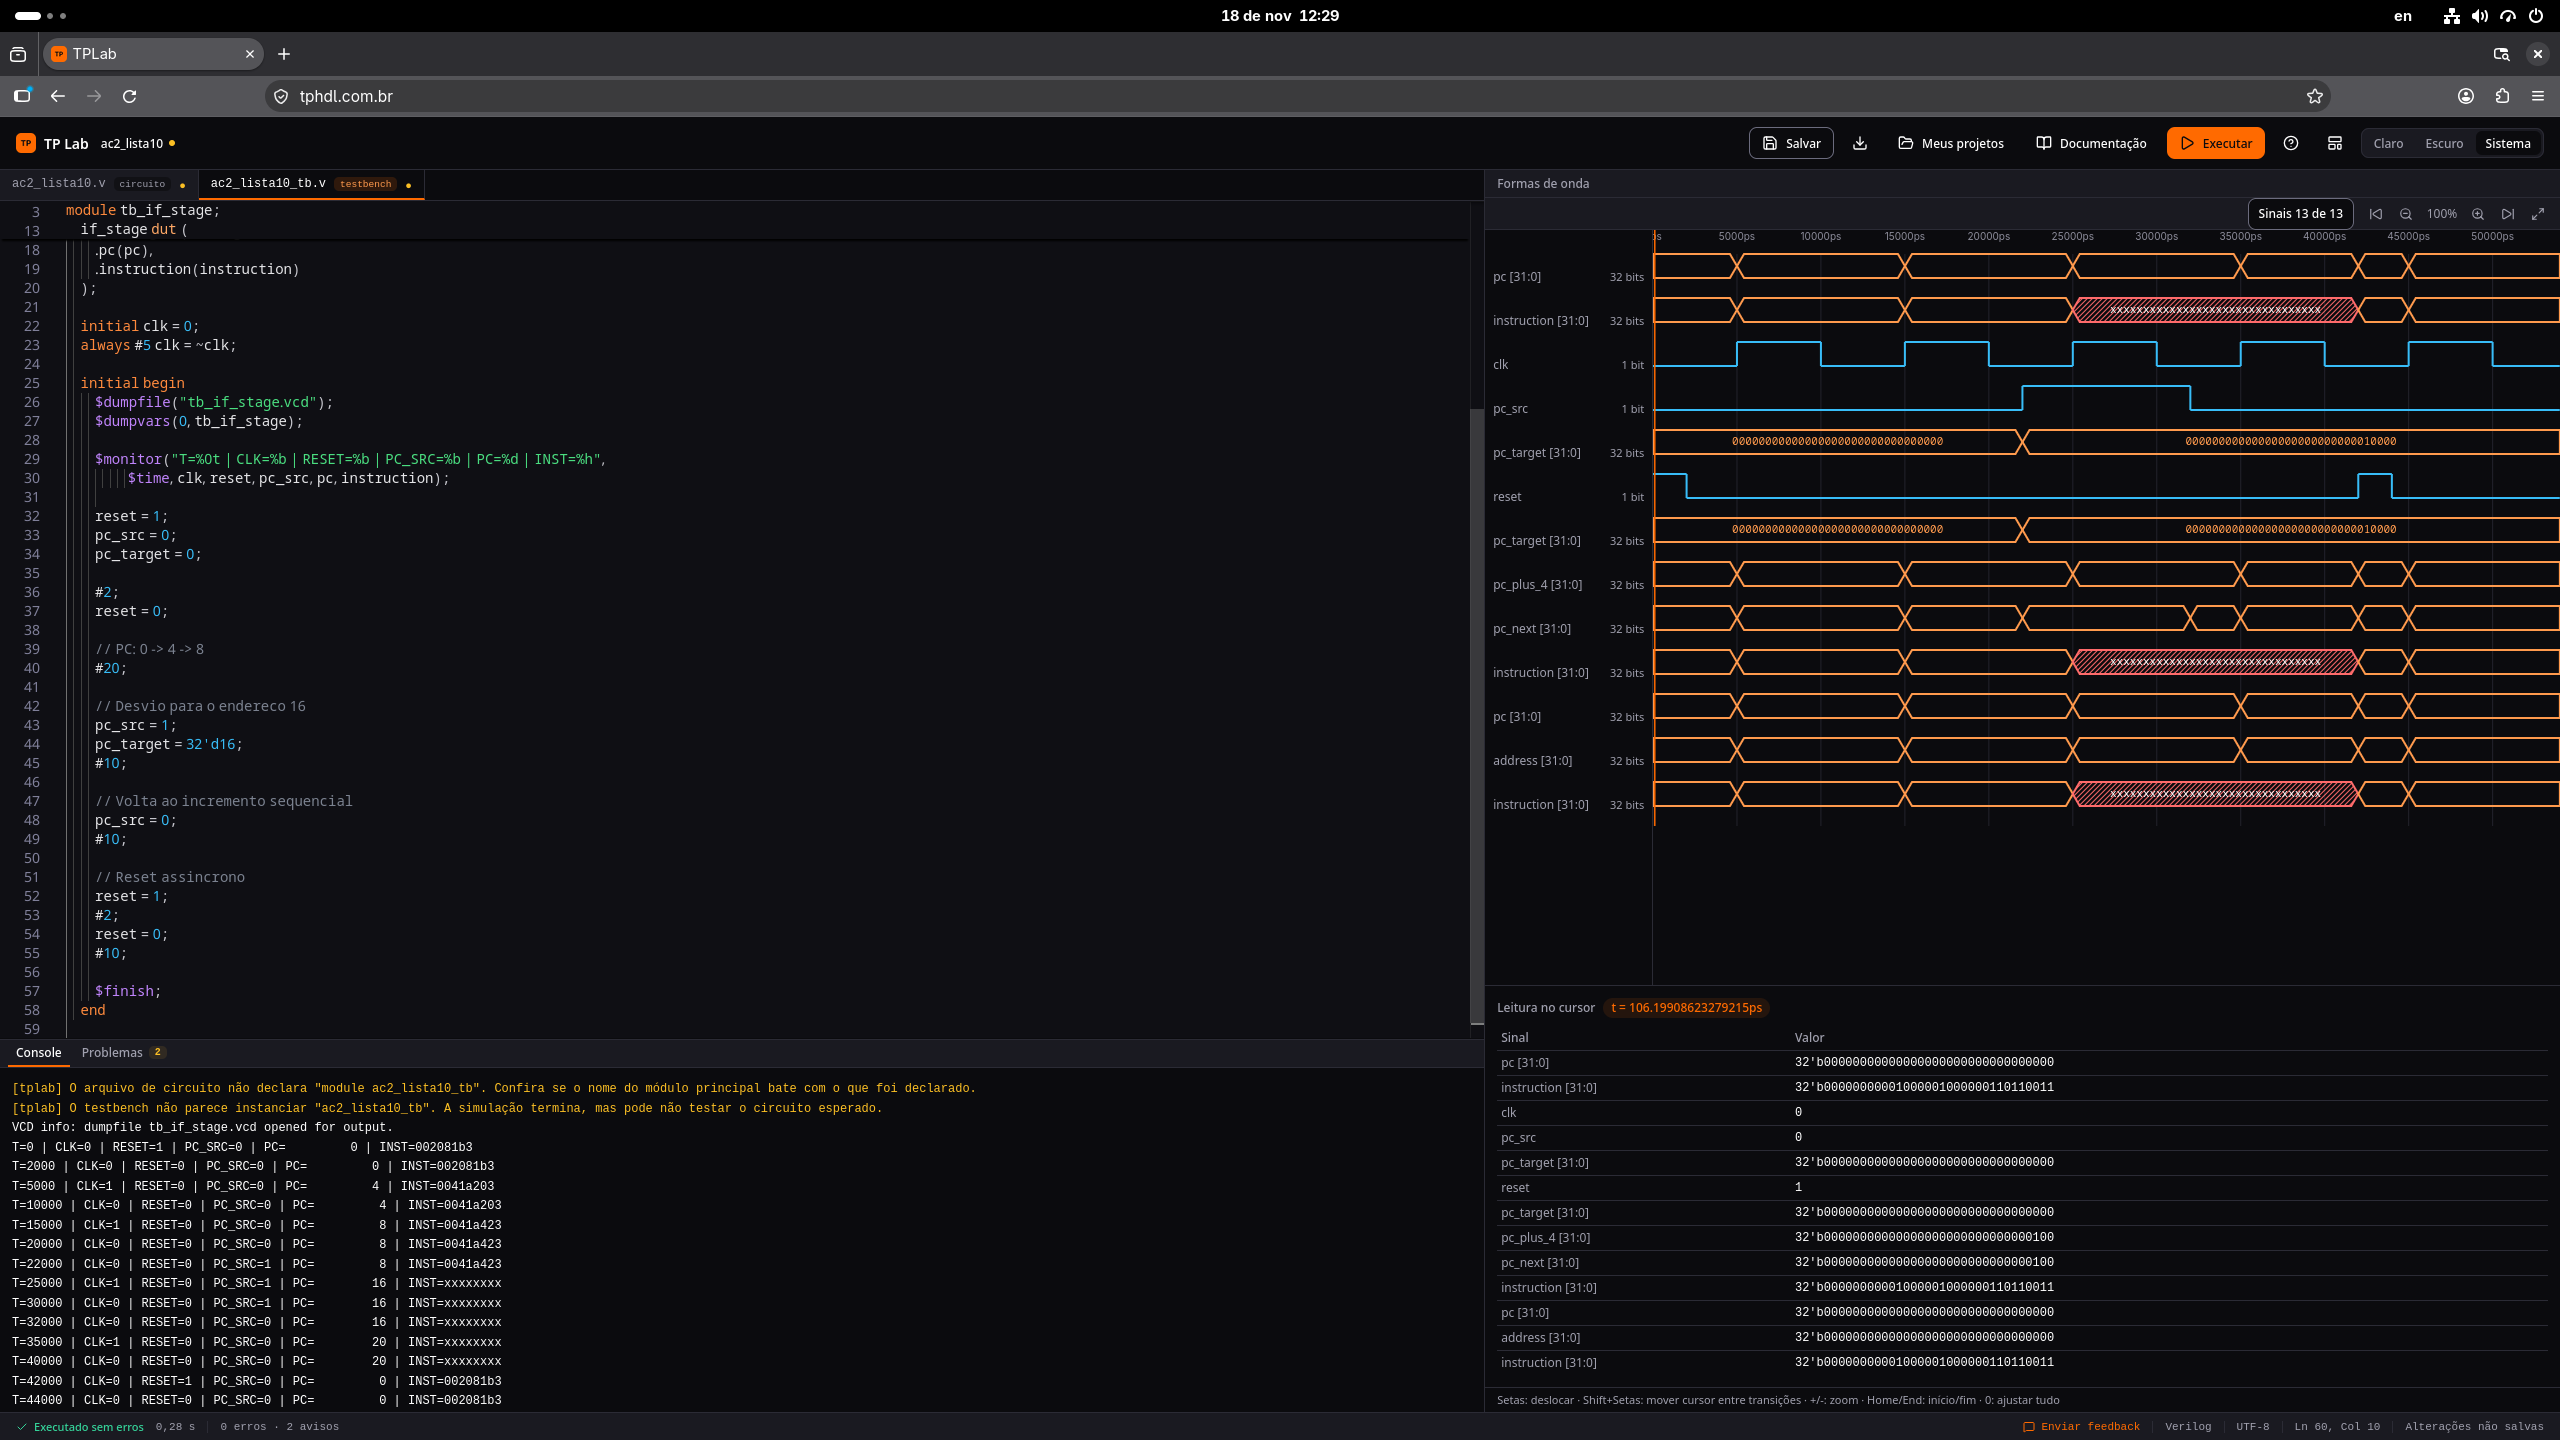
\includegraphics[scale=0.15]{tb_if_stage}
\end{figure}

\clearpage\subsection{Banco de Registradores}
\begin{figure}[h]
    \centering
    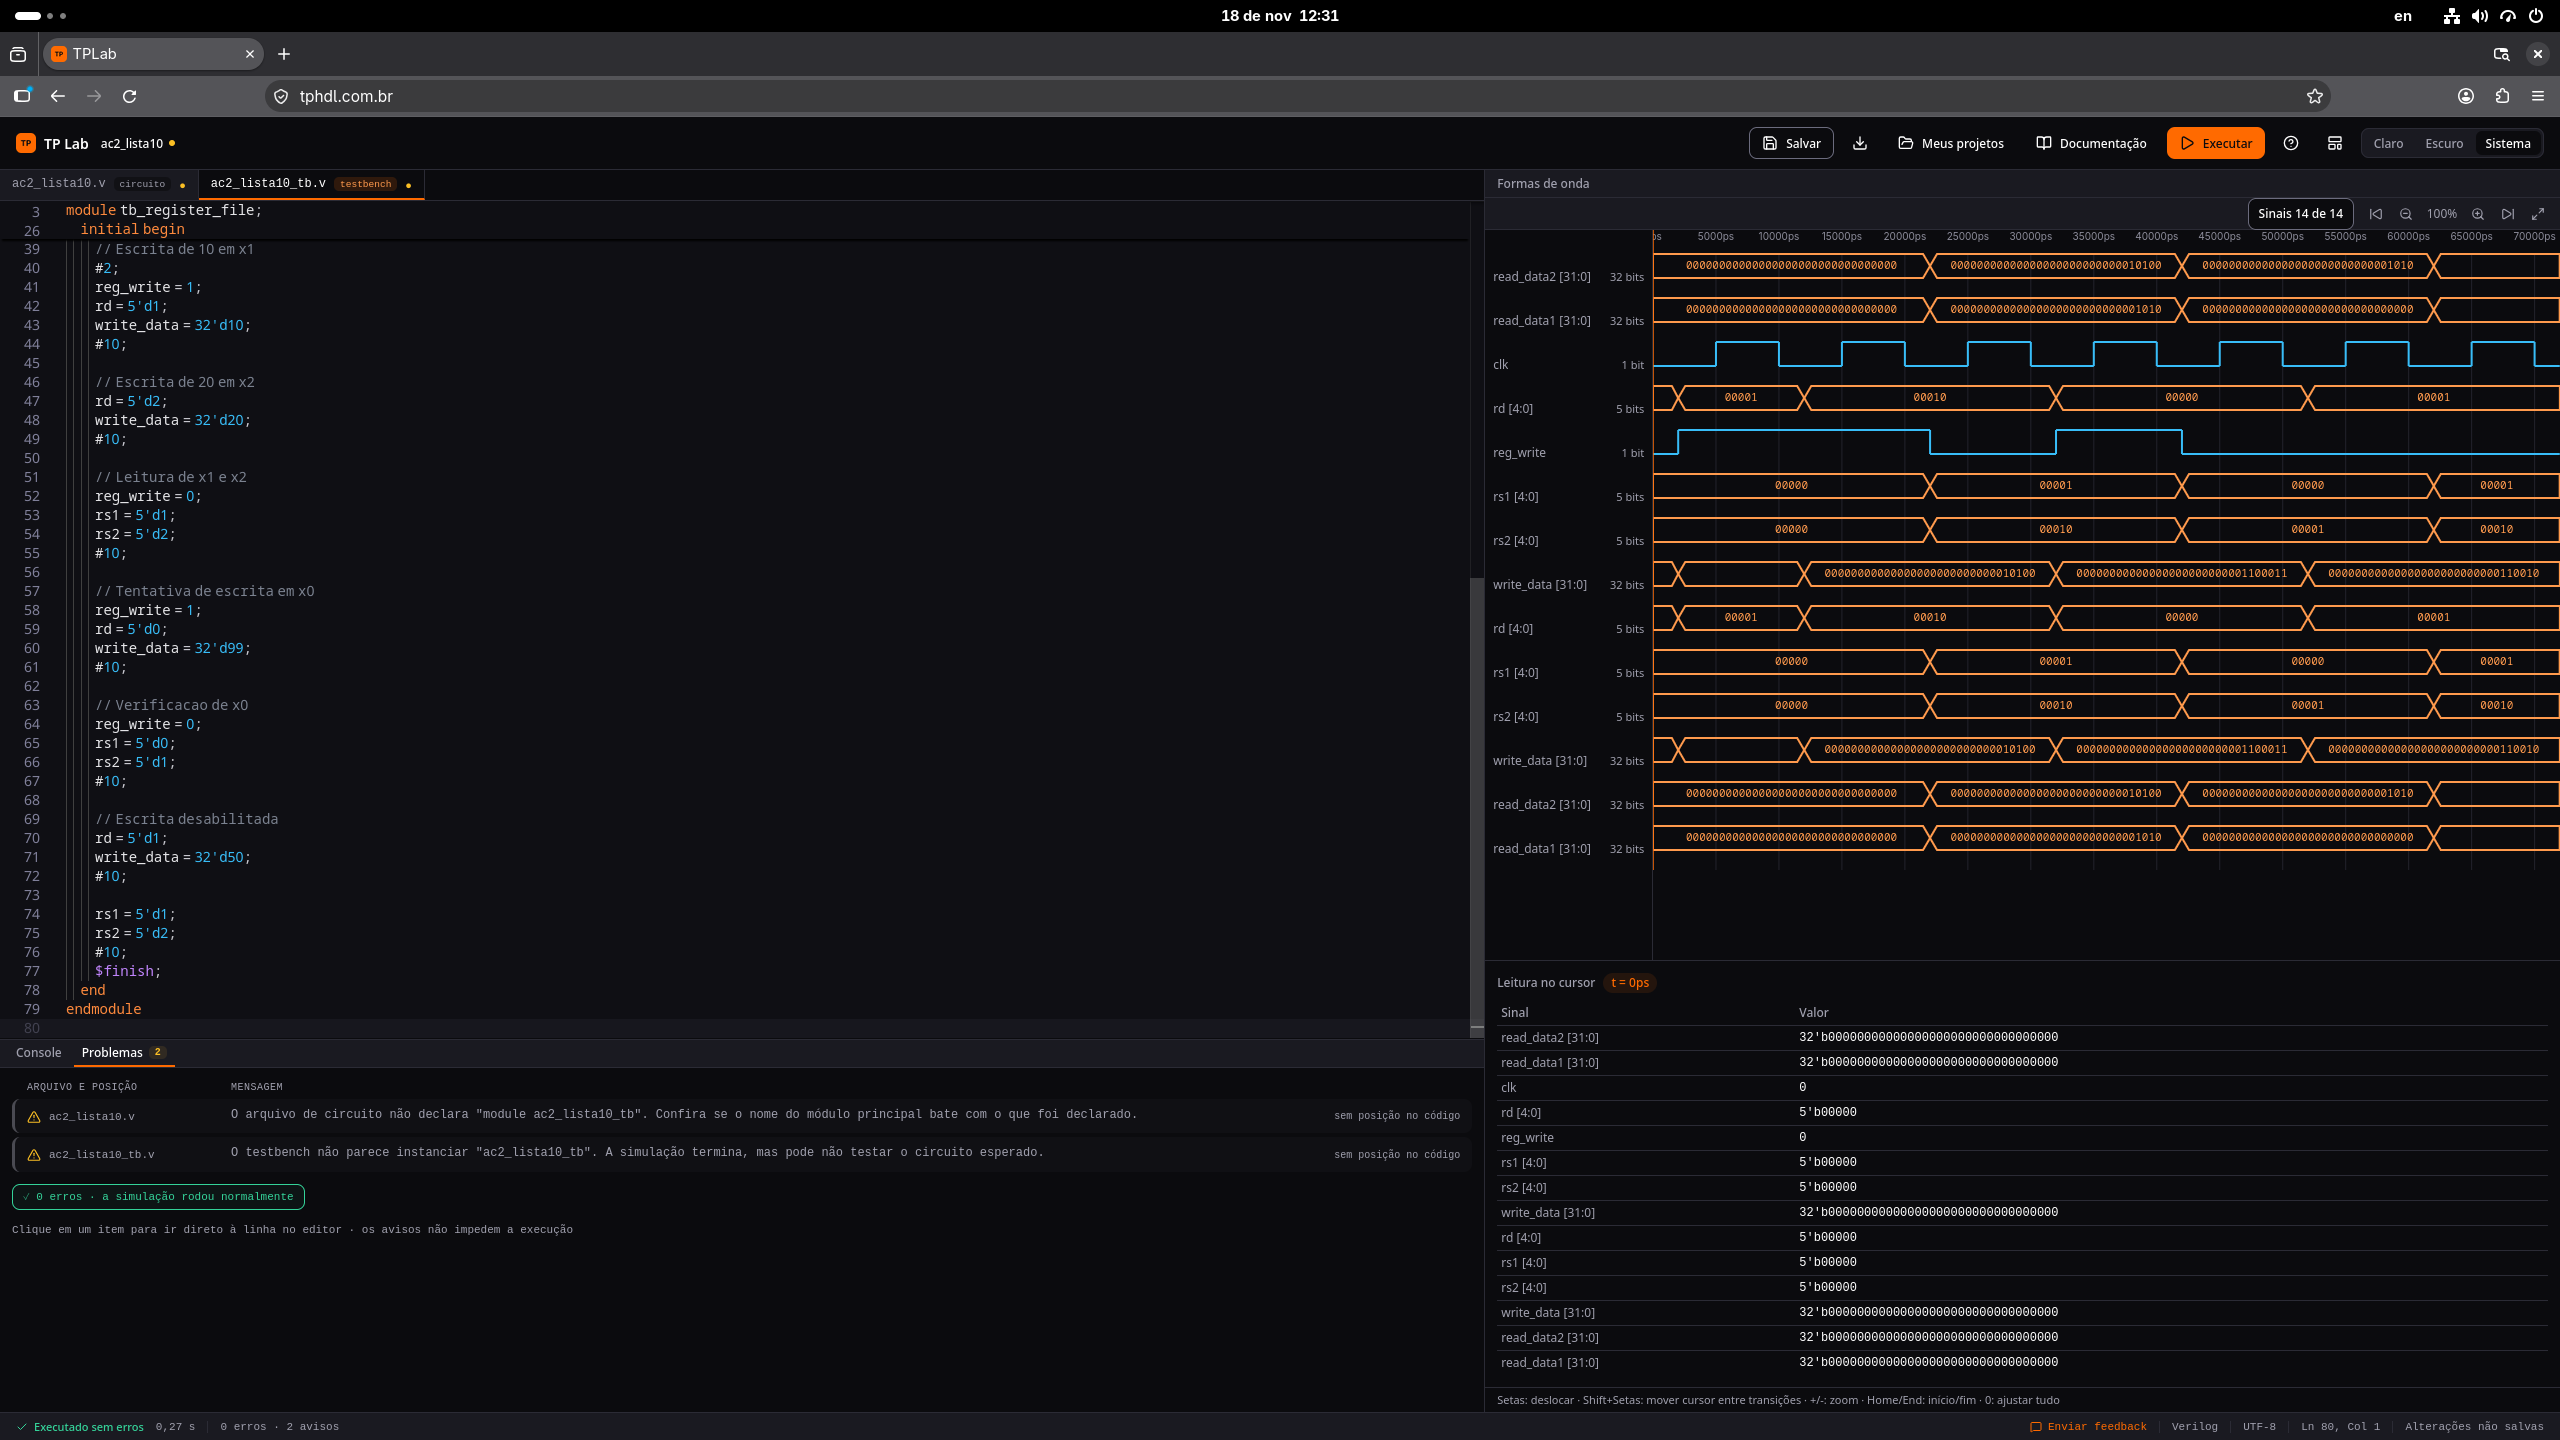
\includegraphics[scale=0.15]{tb_register_file}
\end{figure}

\clearpage\subsection{Gerador de Imediatos}
\begin{figure}[h]
    \centering
    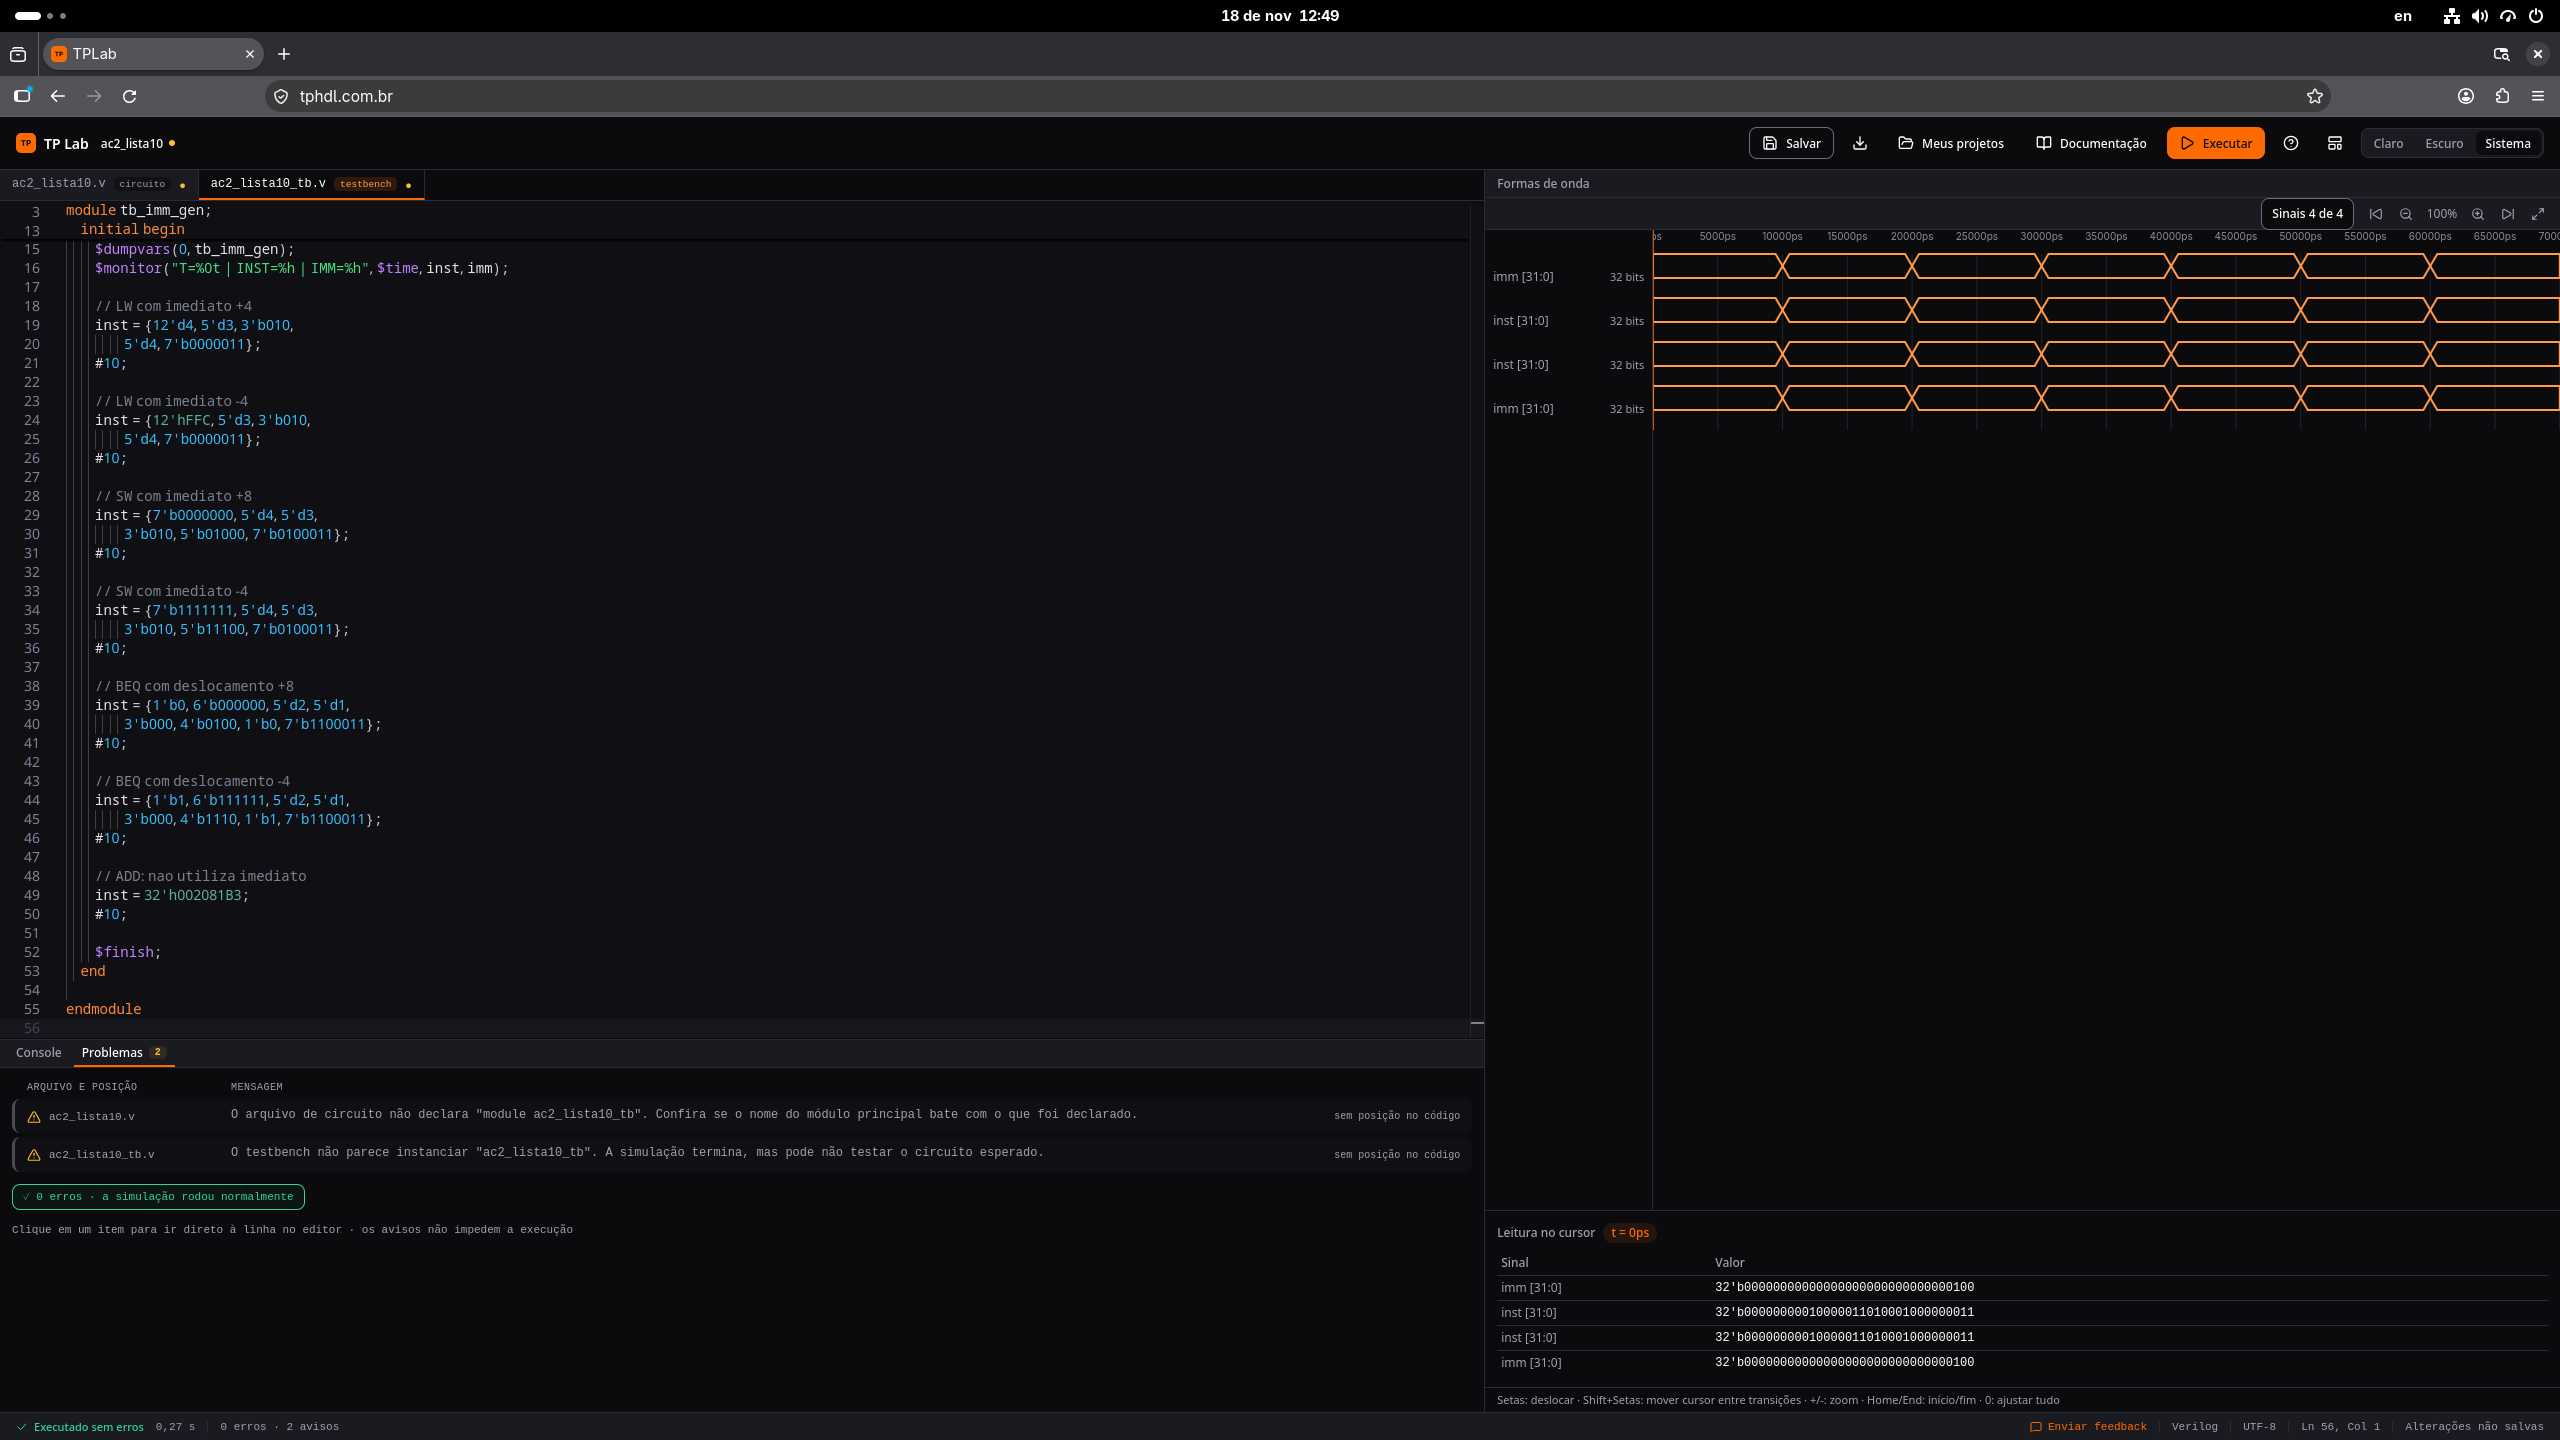
\includegraphics[scale=0.15]{tb_imm_gen}
\end{figure}

\clearpage\subsection{Módulo de Decodificação}
\begin{figure}[h]
    \centering
    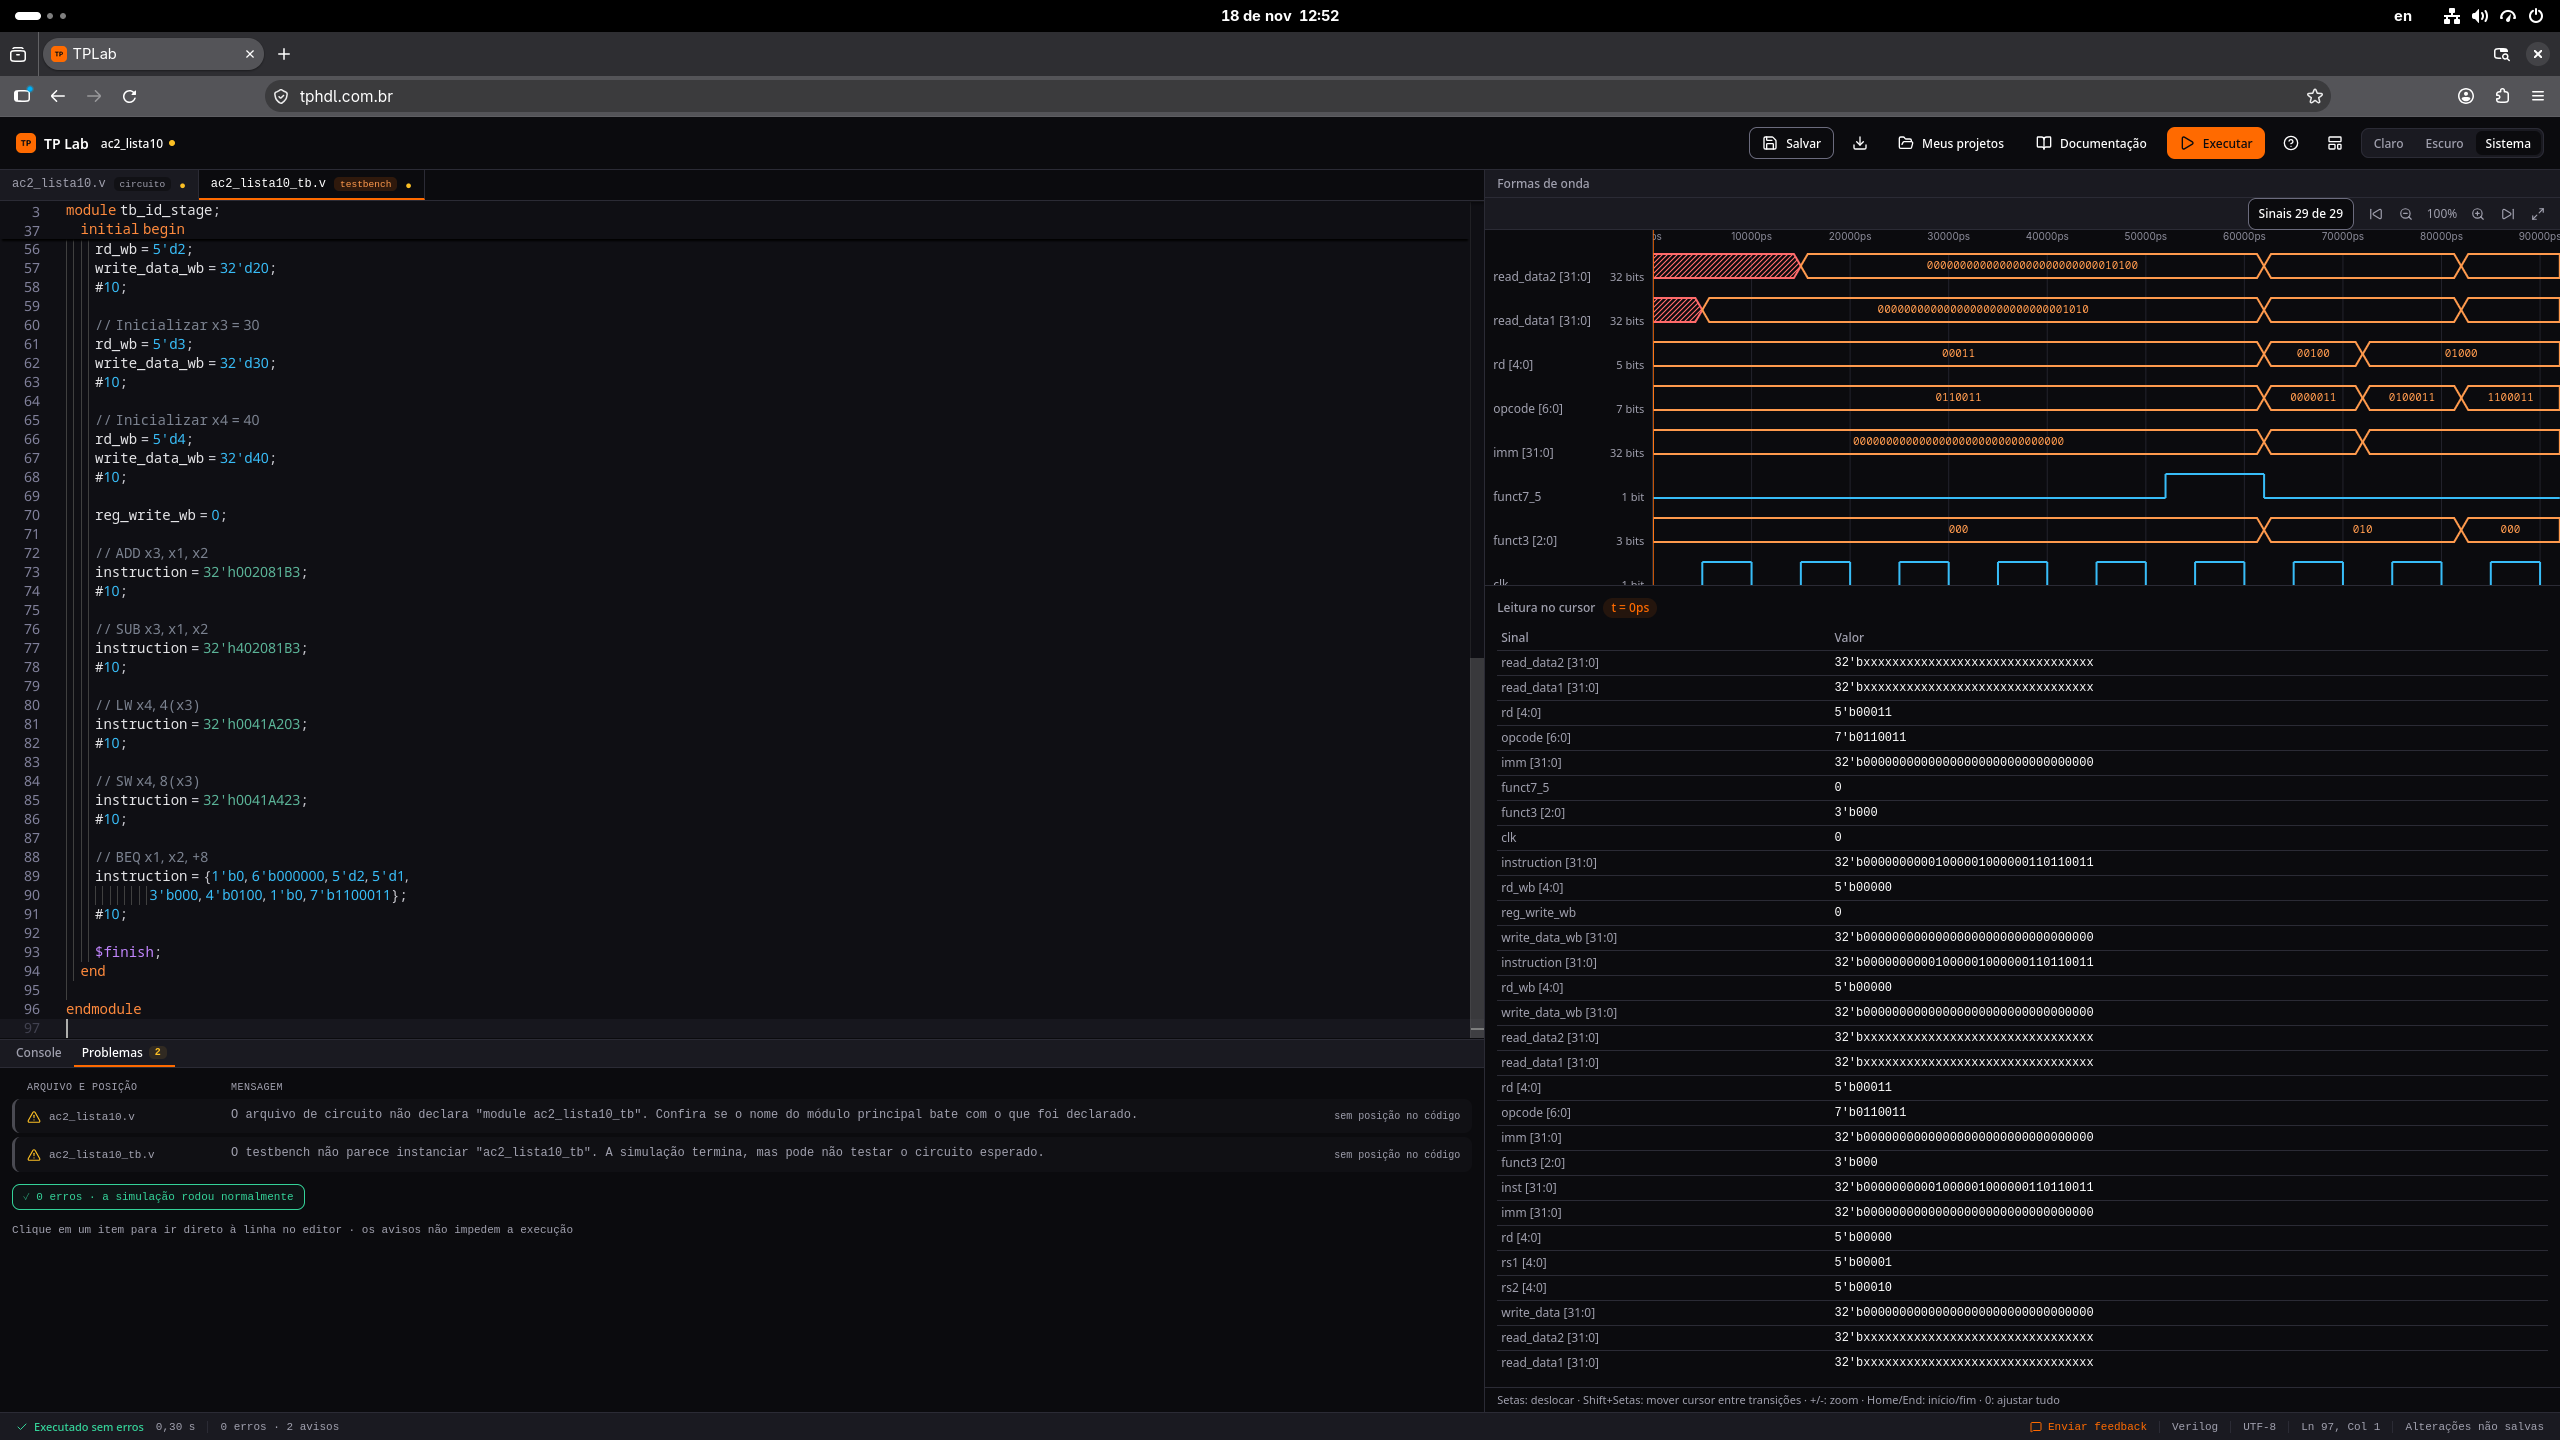
\includegraphics[scale=0.15]{tb_id_stage}
\end{figure}

\clearpage\subsection{Unidade de Controle}
\begin{figure}[h]
    \centering
    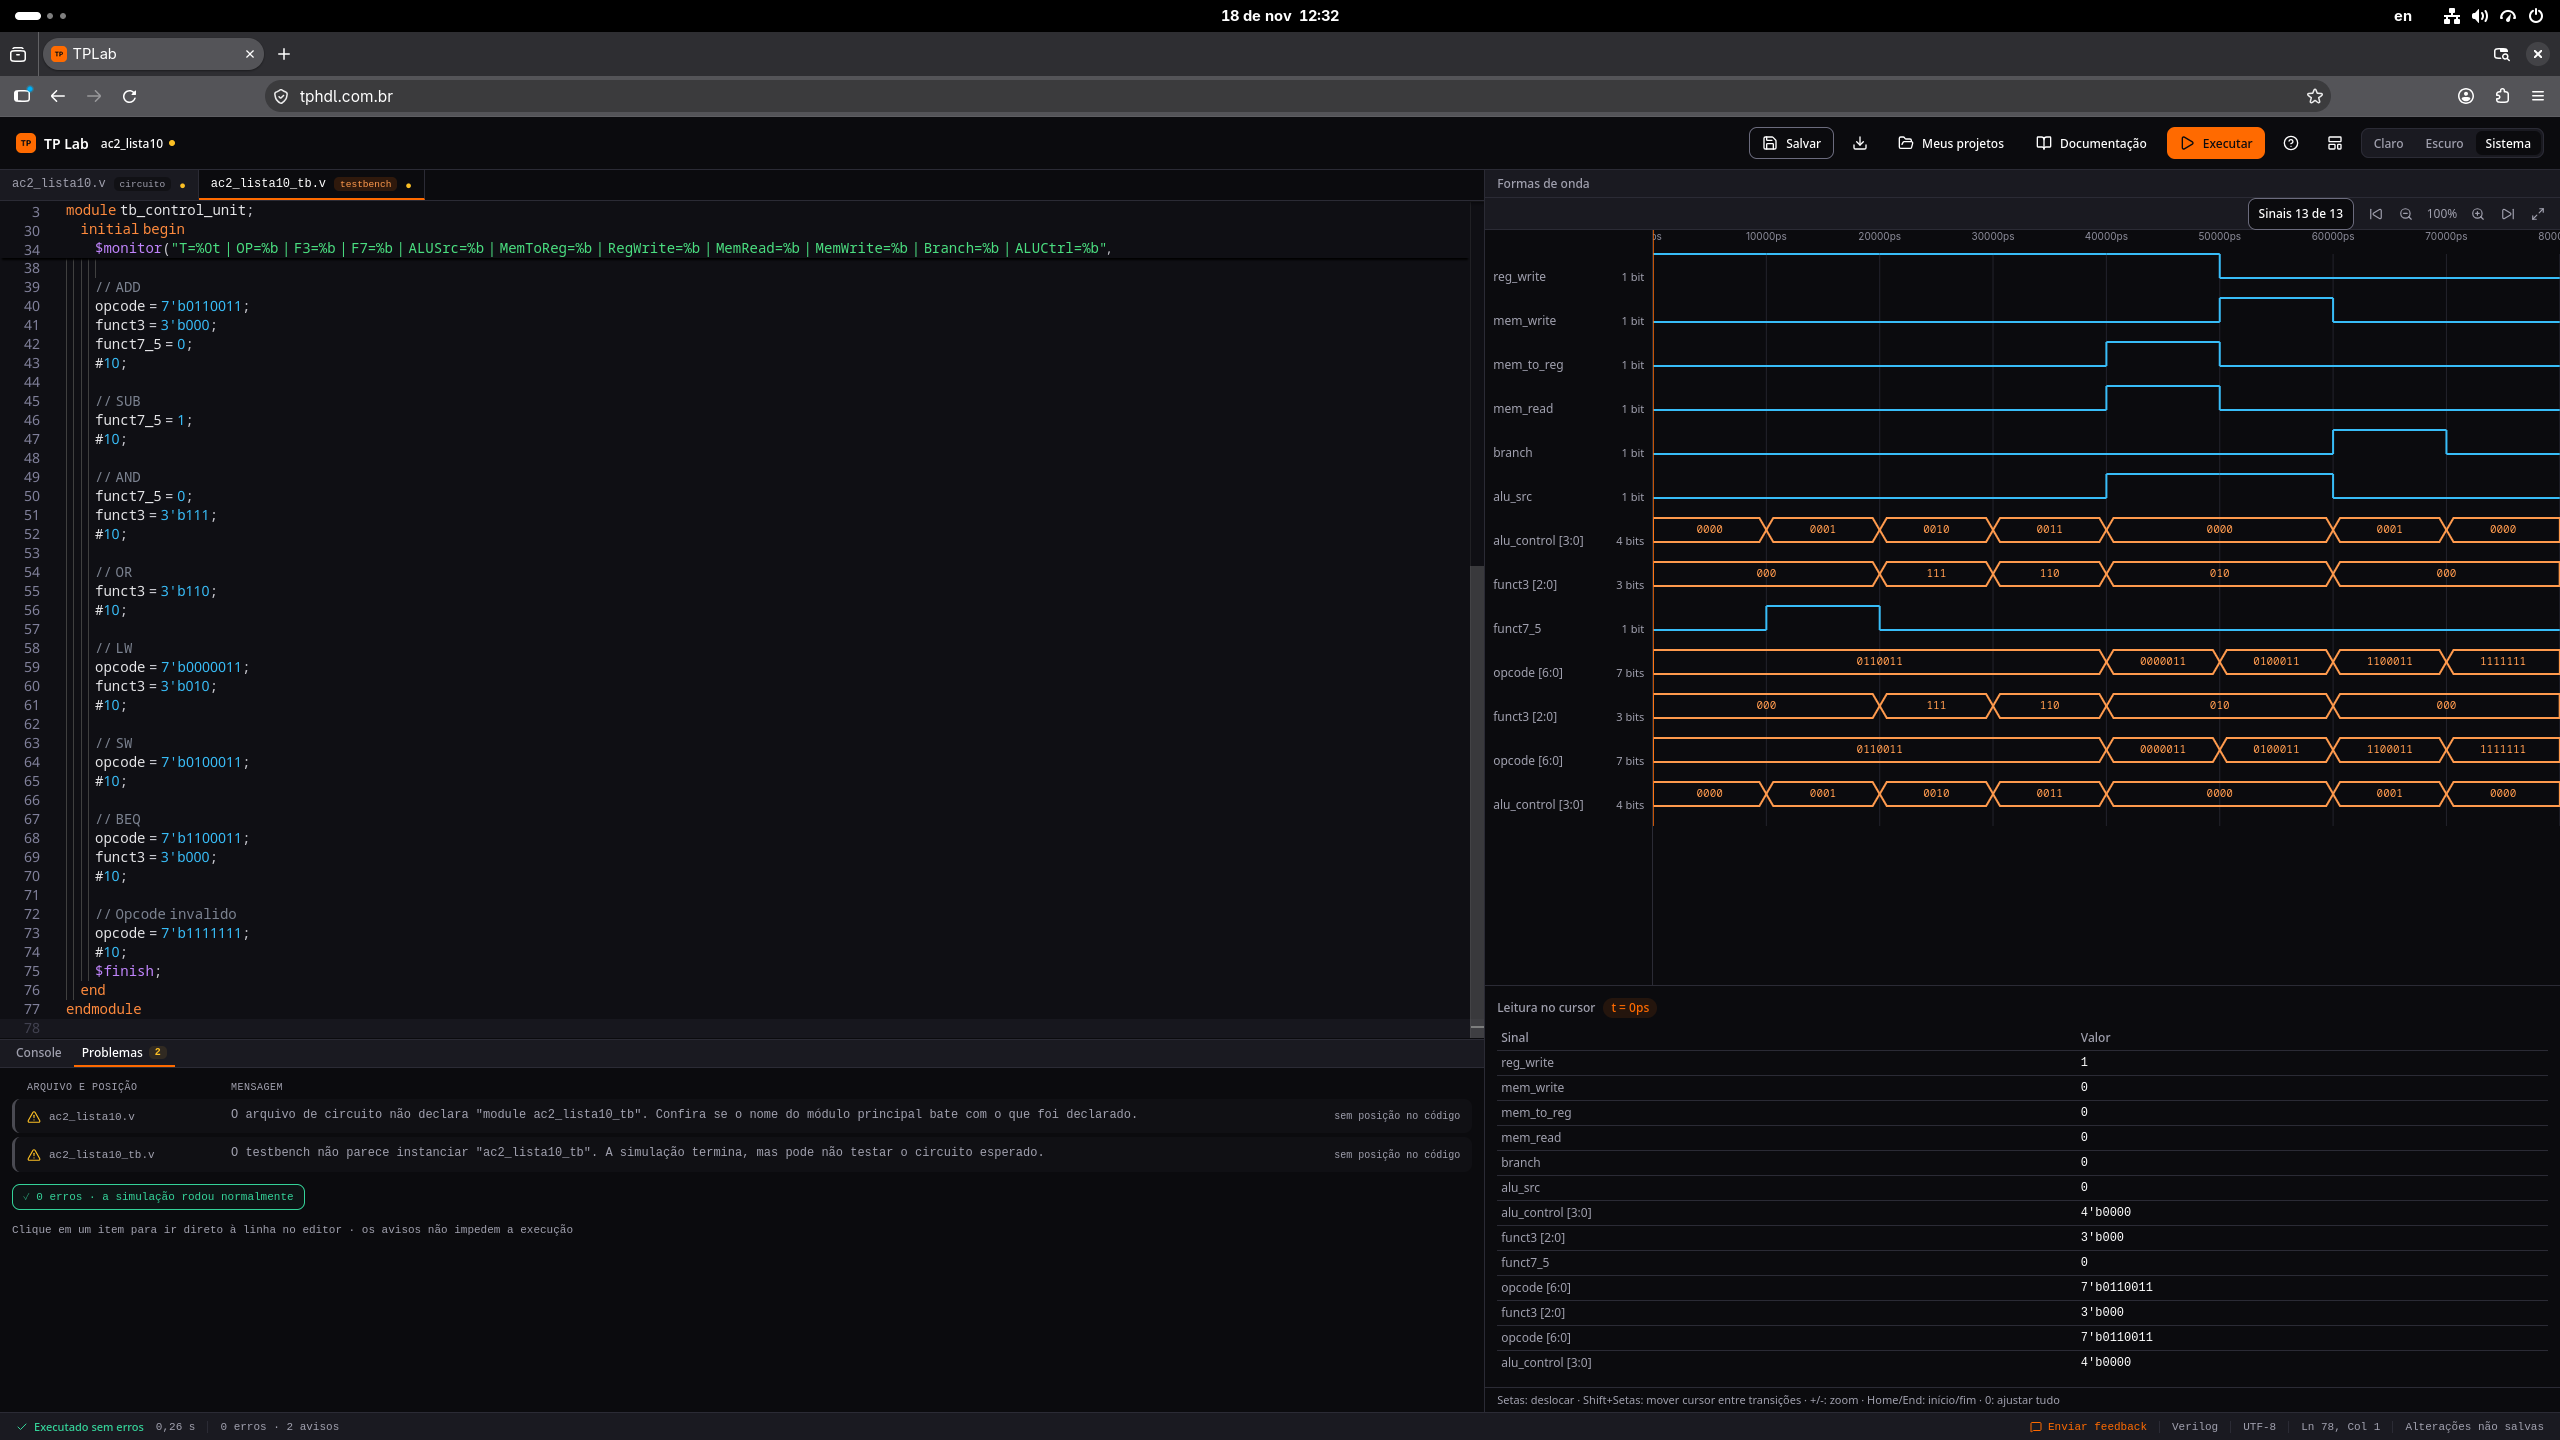
\includegraphics[scale=0.15]{tb_control_unit}
\end{figure}

\clearpage\subsection{Execution}
\begin{figure}[h]
    \centering
    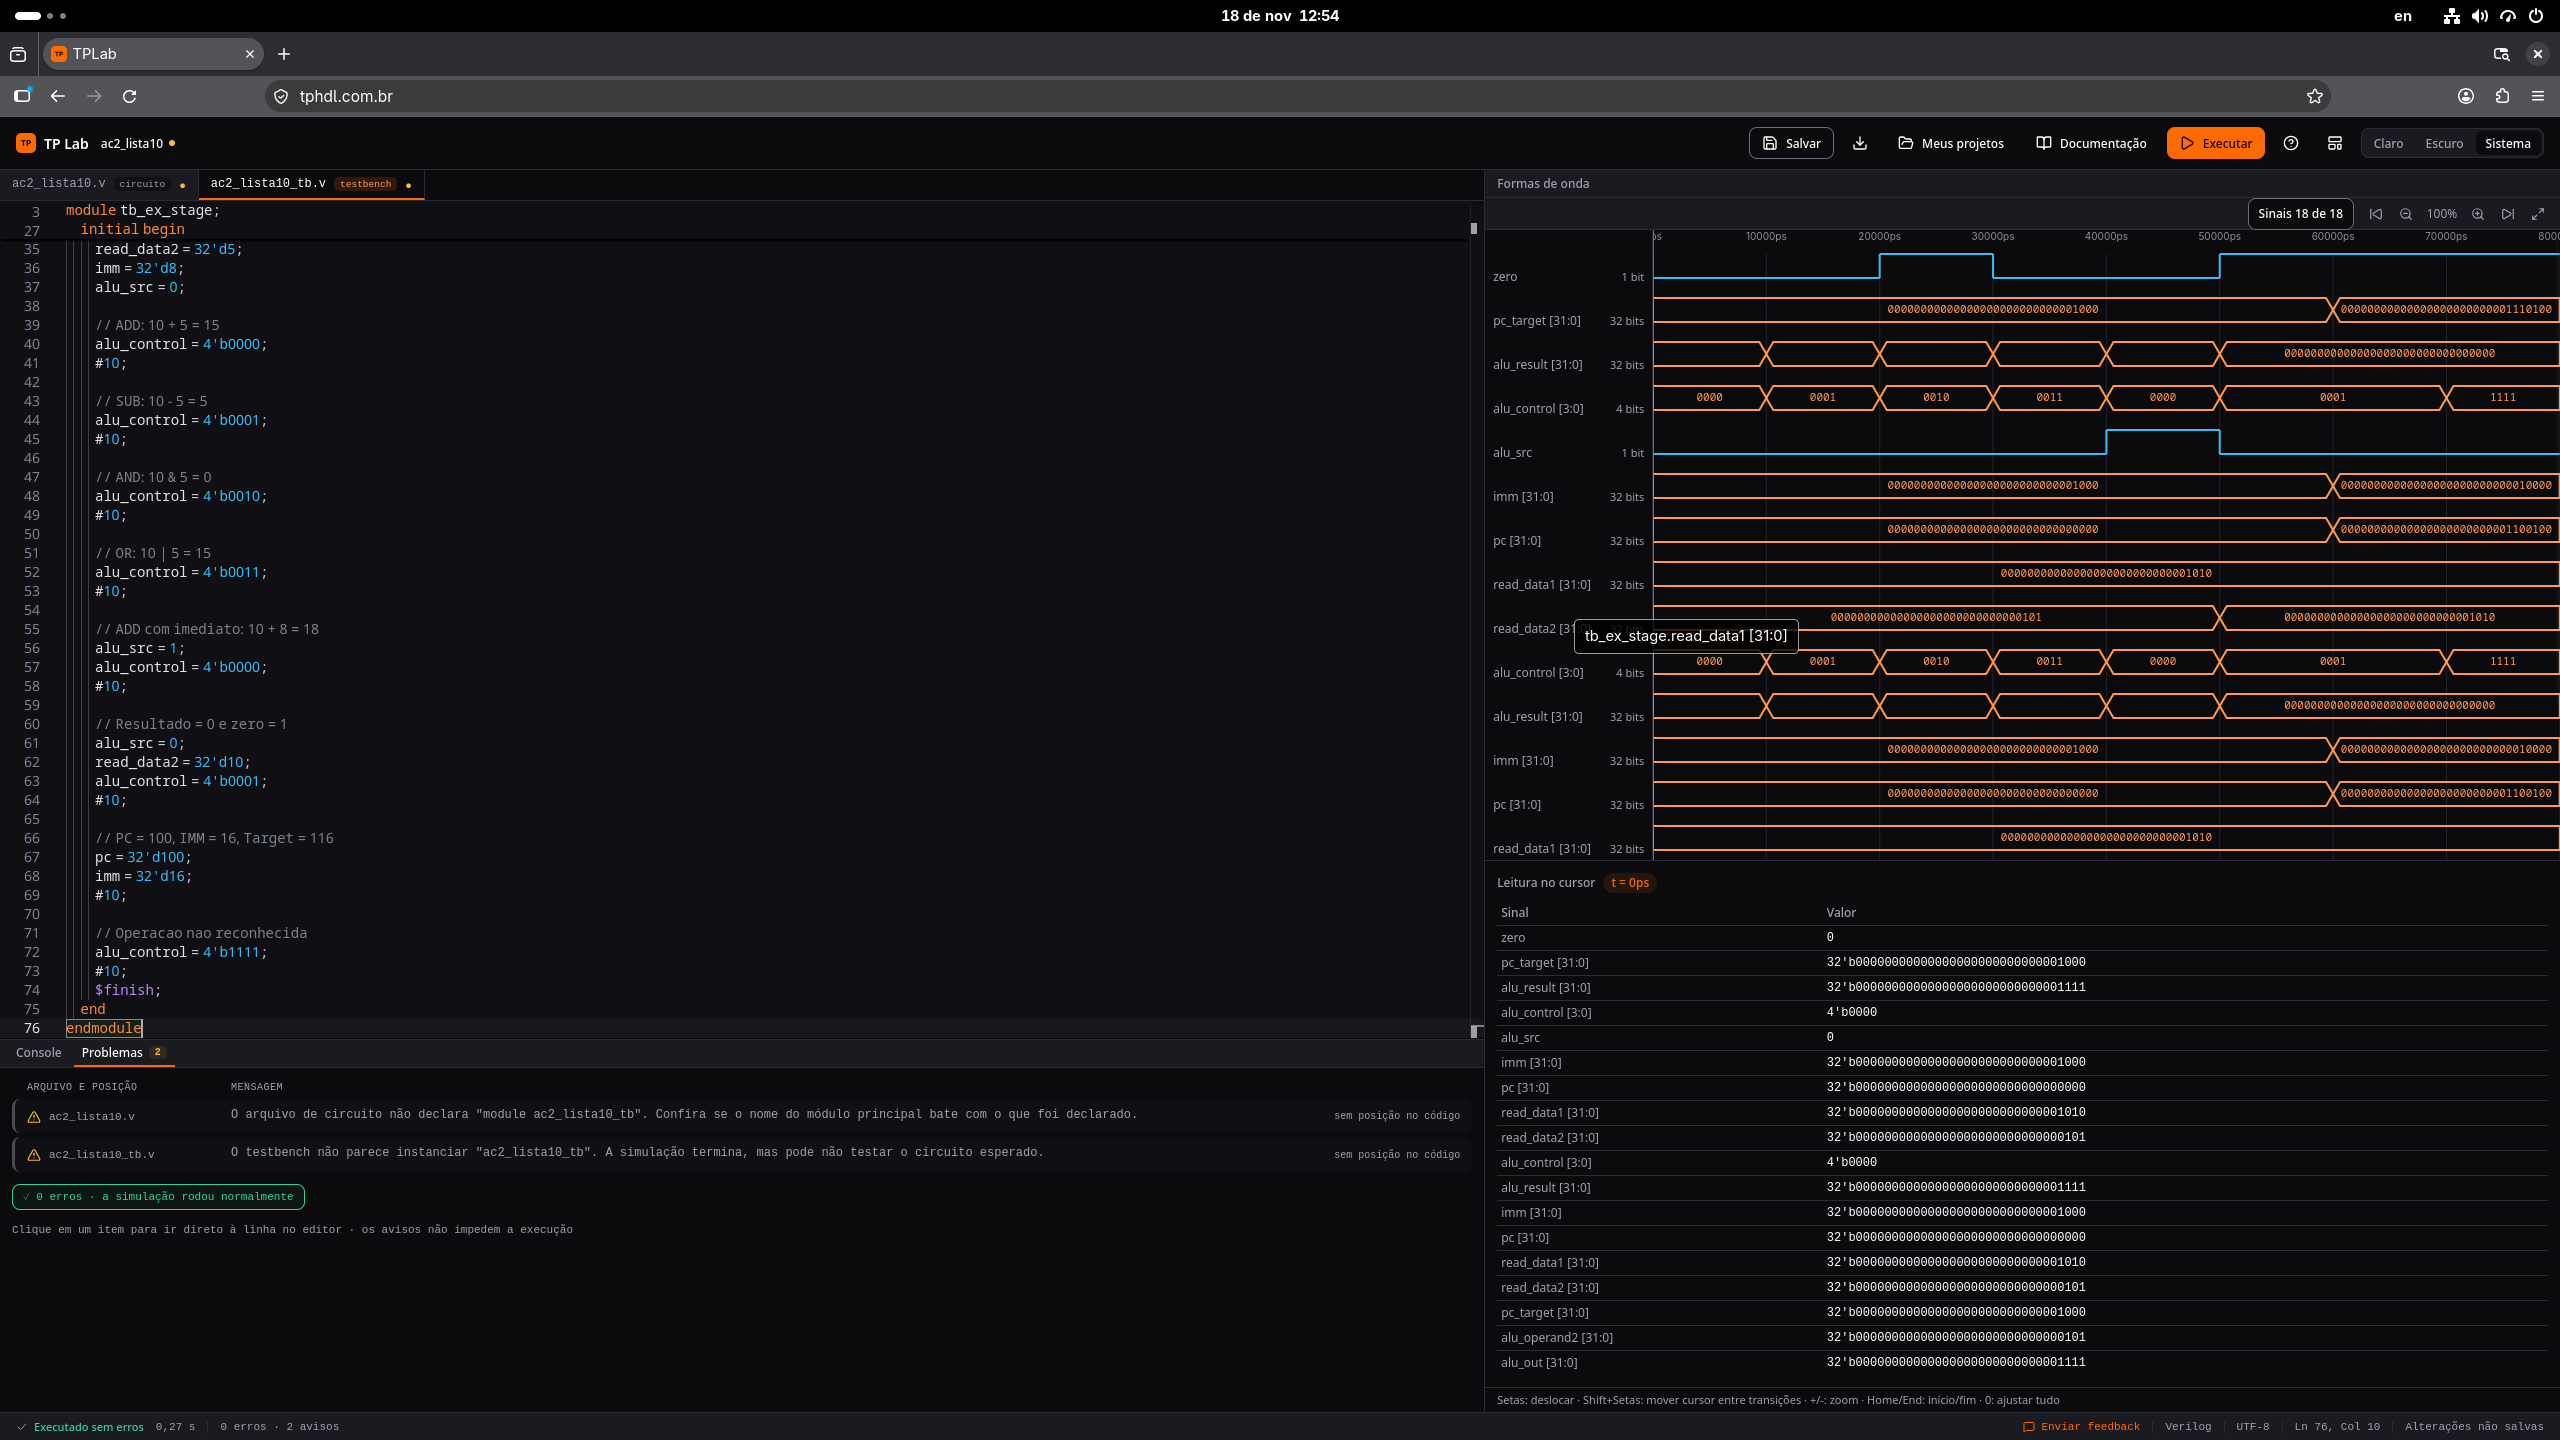
\includegraphics[scale=0.15]{tb_ex_stage}
\end{figure}

\clearpage\subsection{Memory Unit}
\begin{figure}[h]
    \centering
    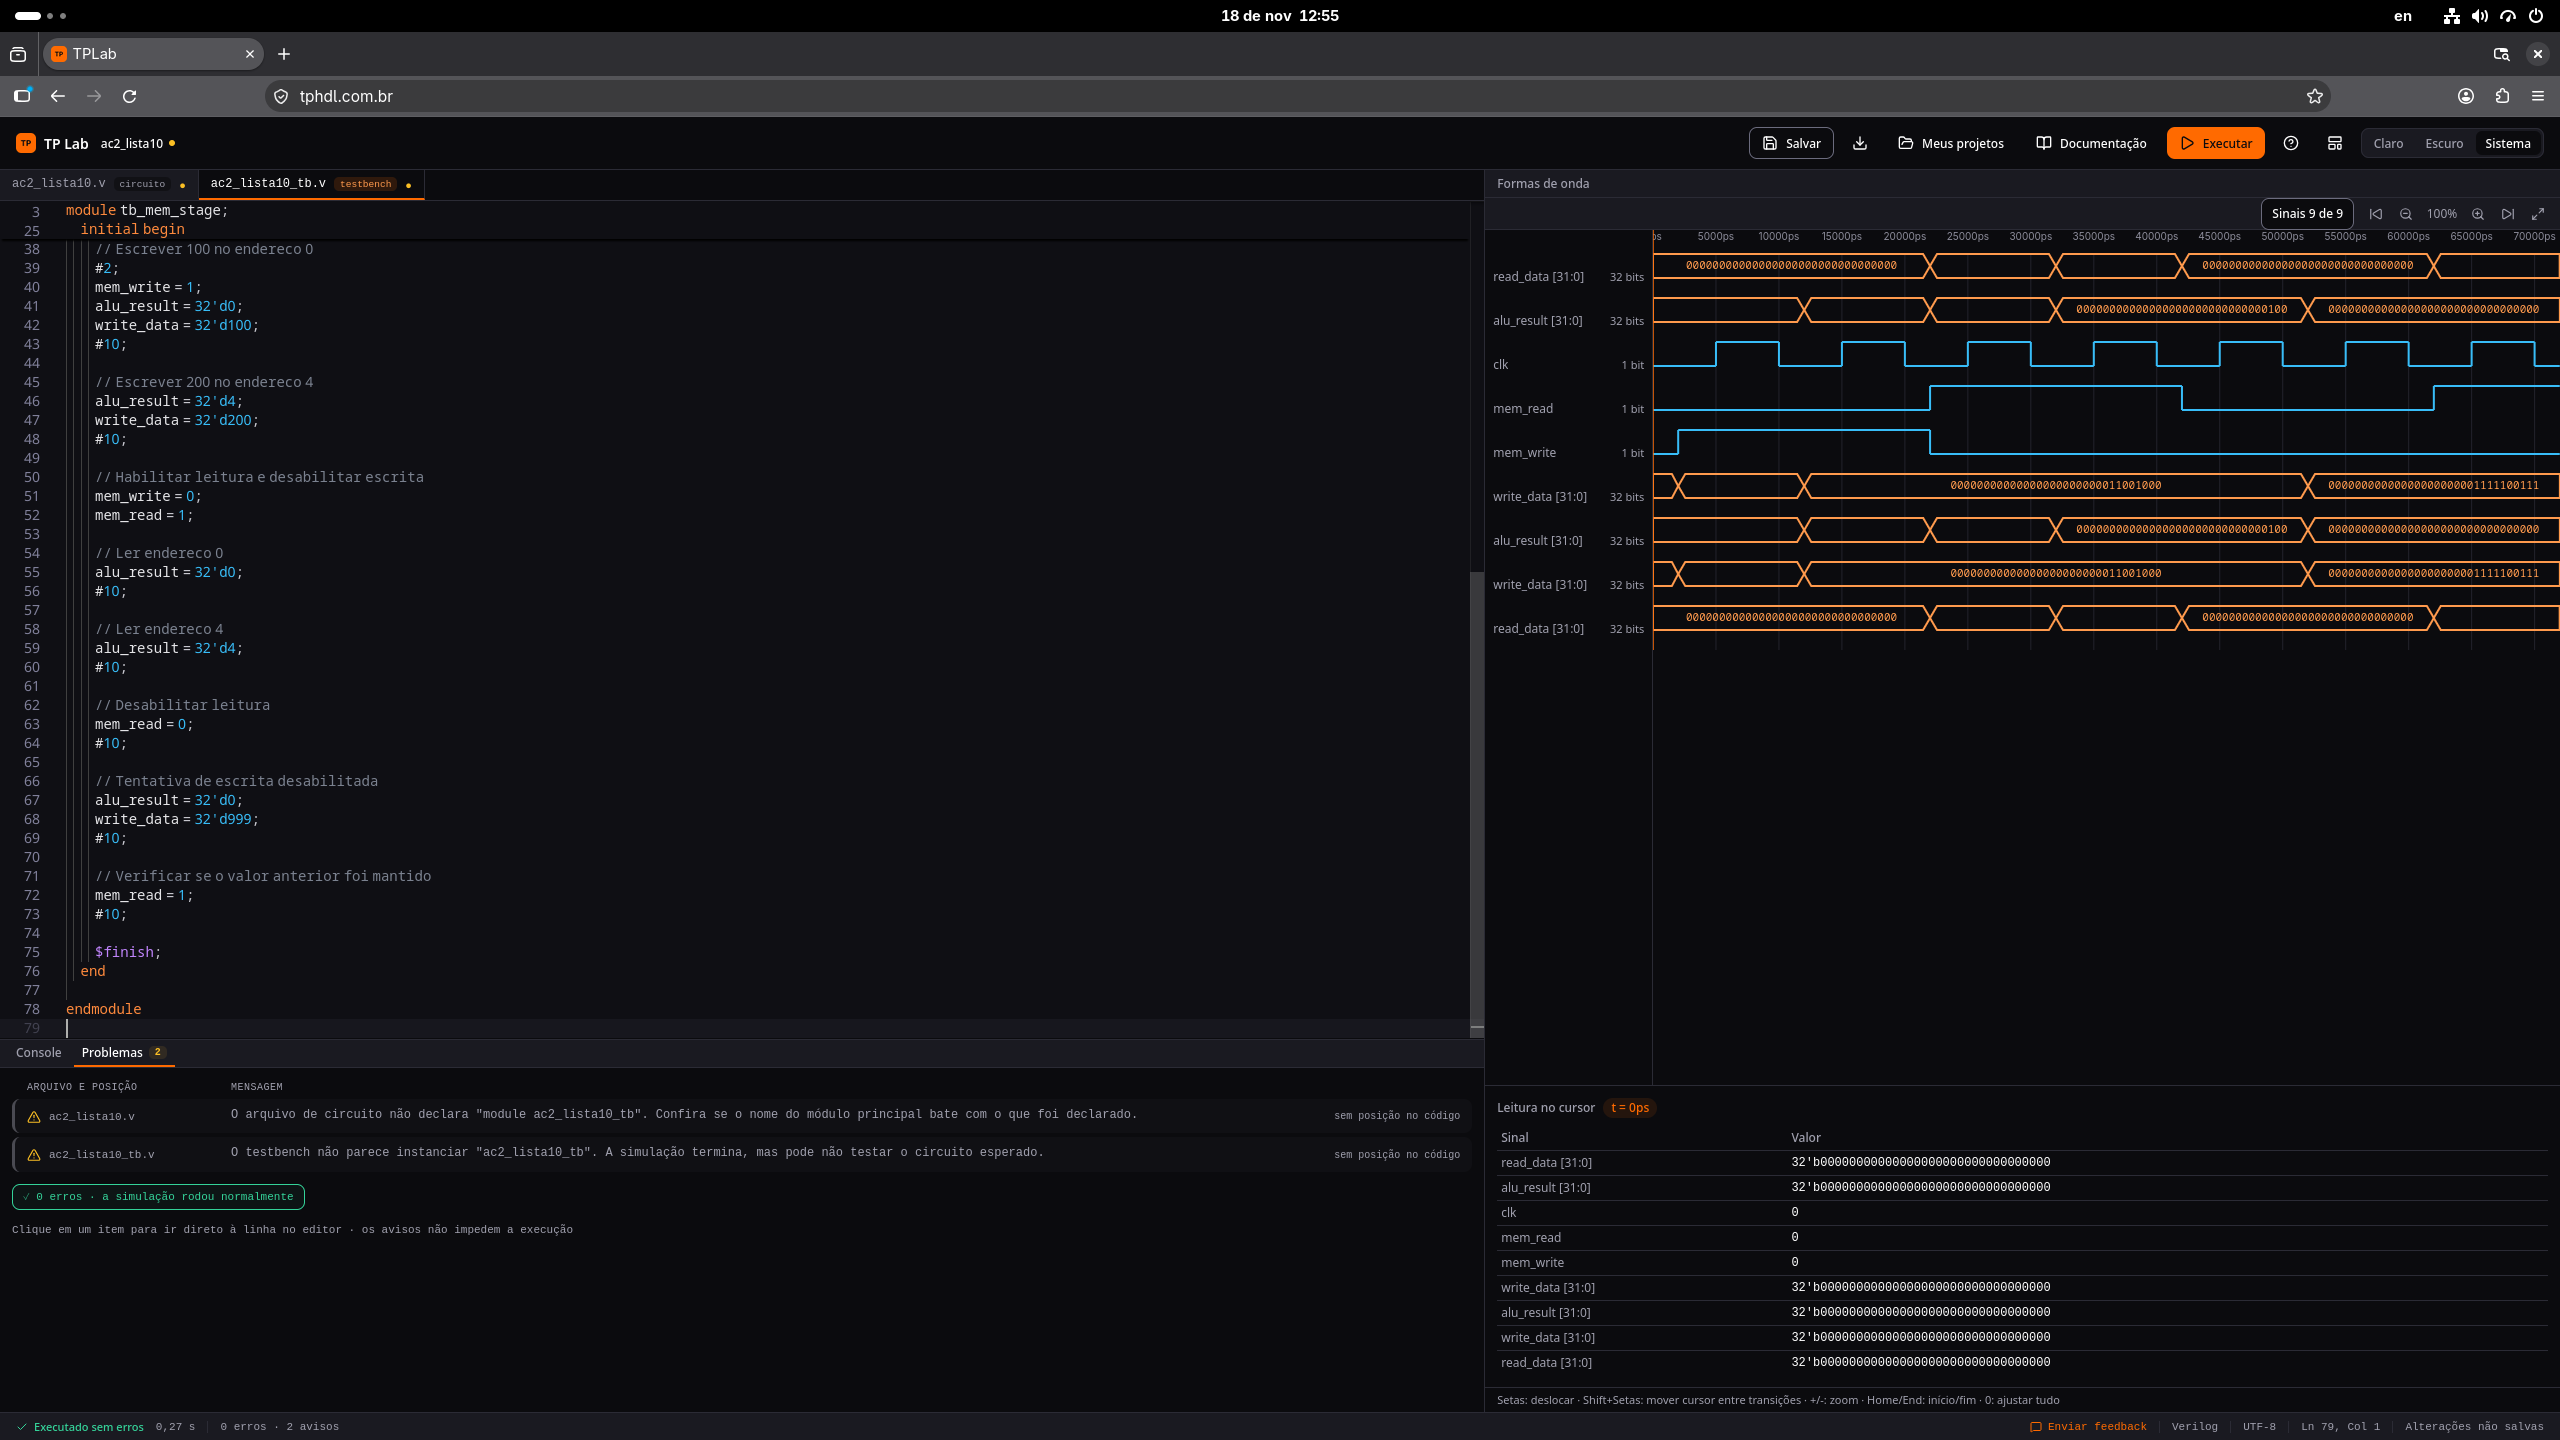
\includegraphics[scale=0.15]{tb_mem_stage}
\end{figure}

\clearpage\subsection{Write Back}
\begin{figure}[h]
    \centering
    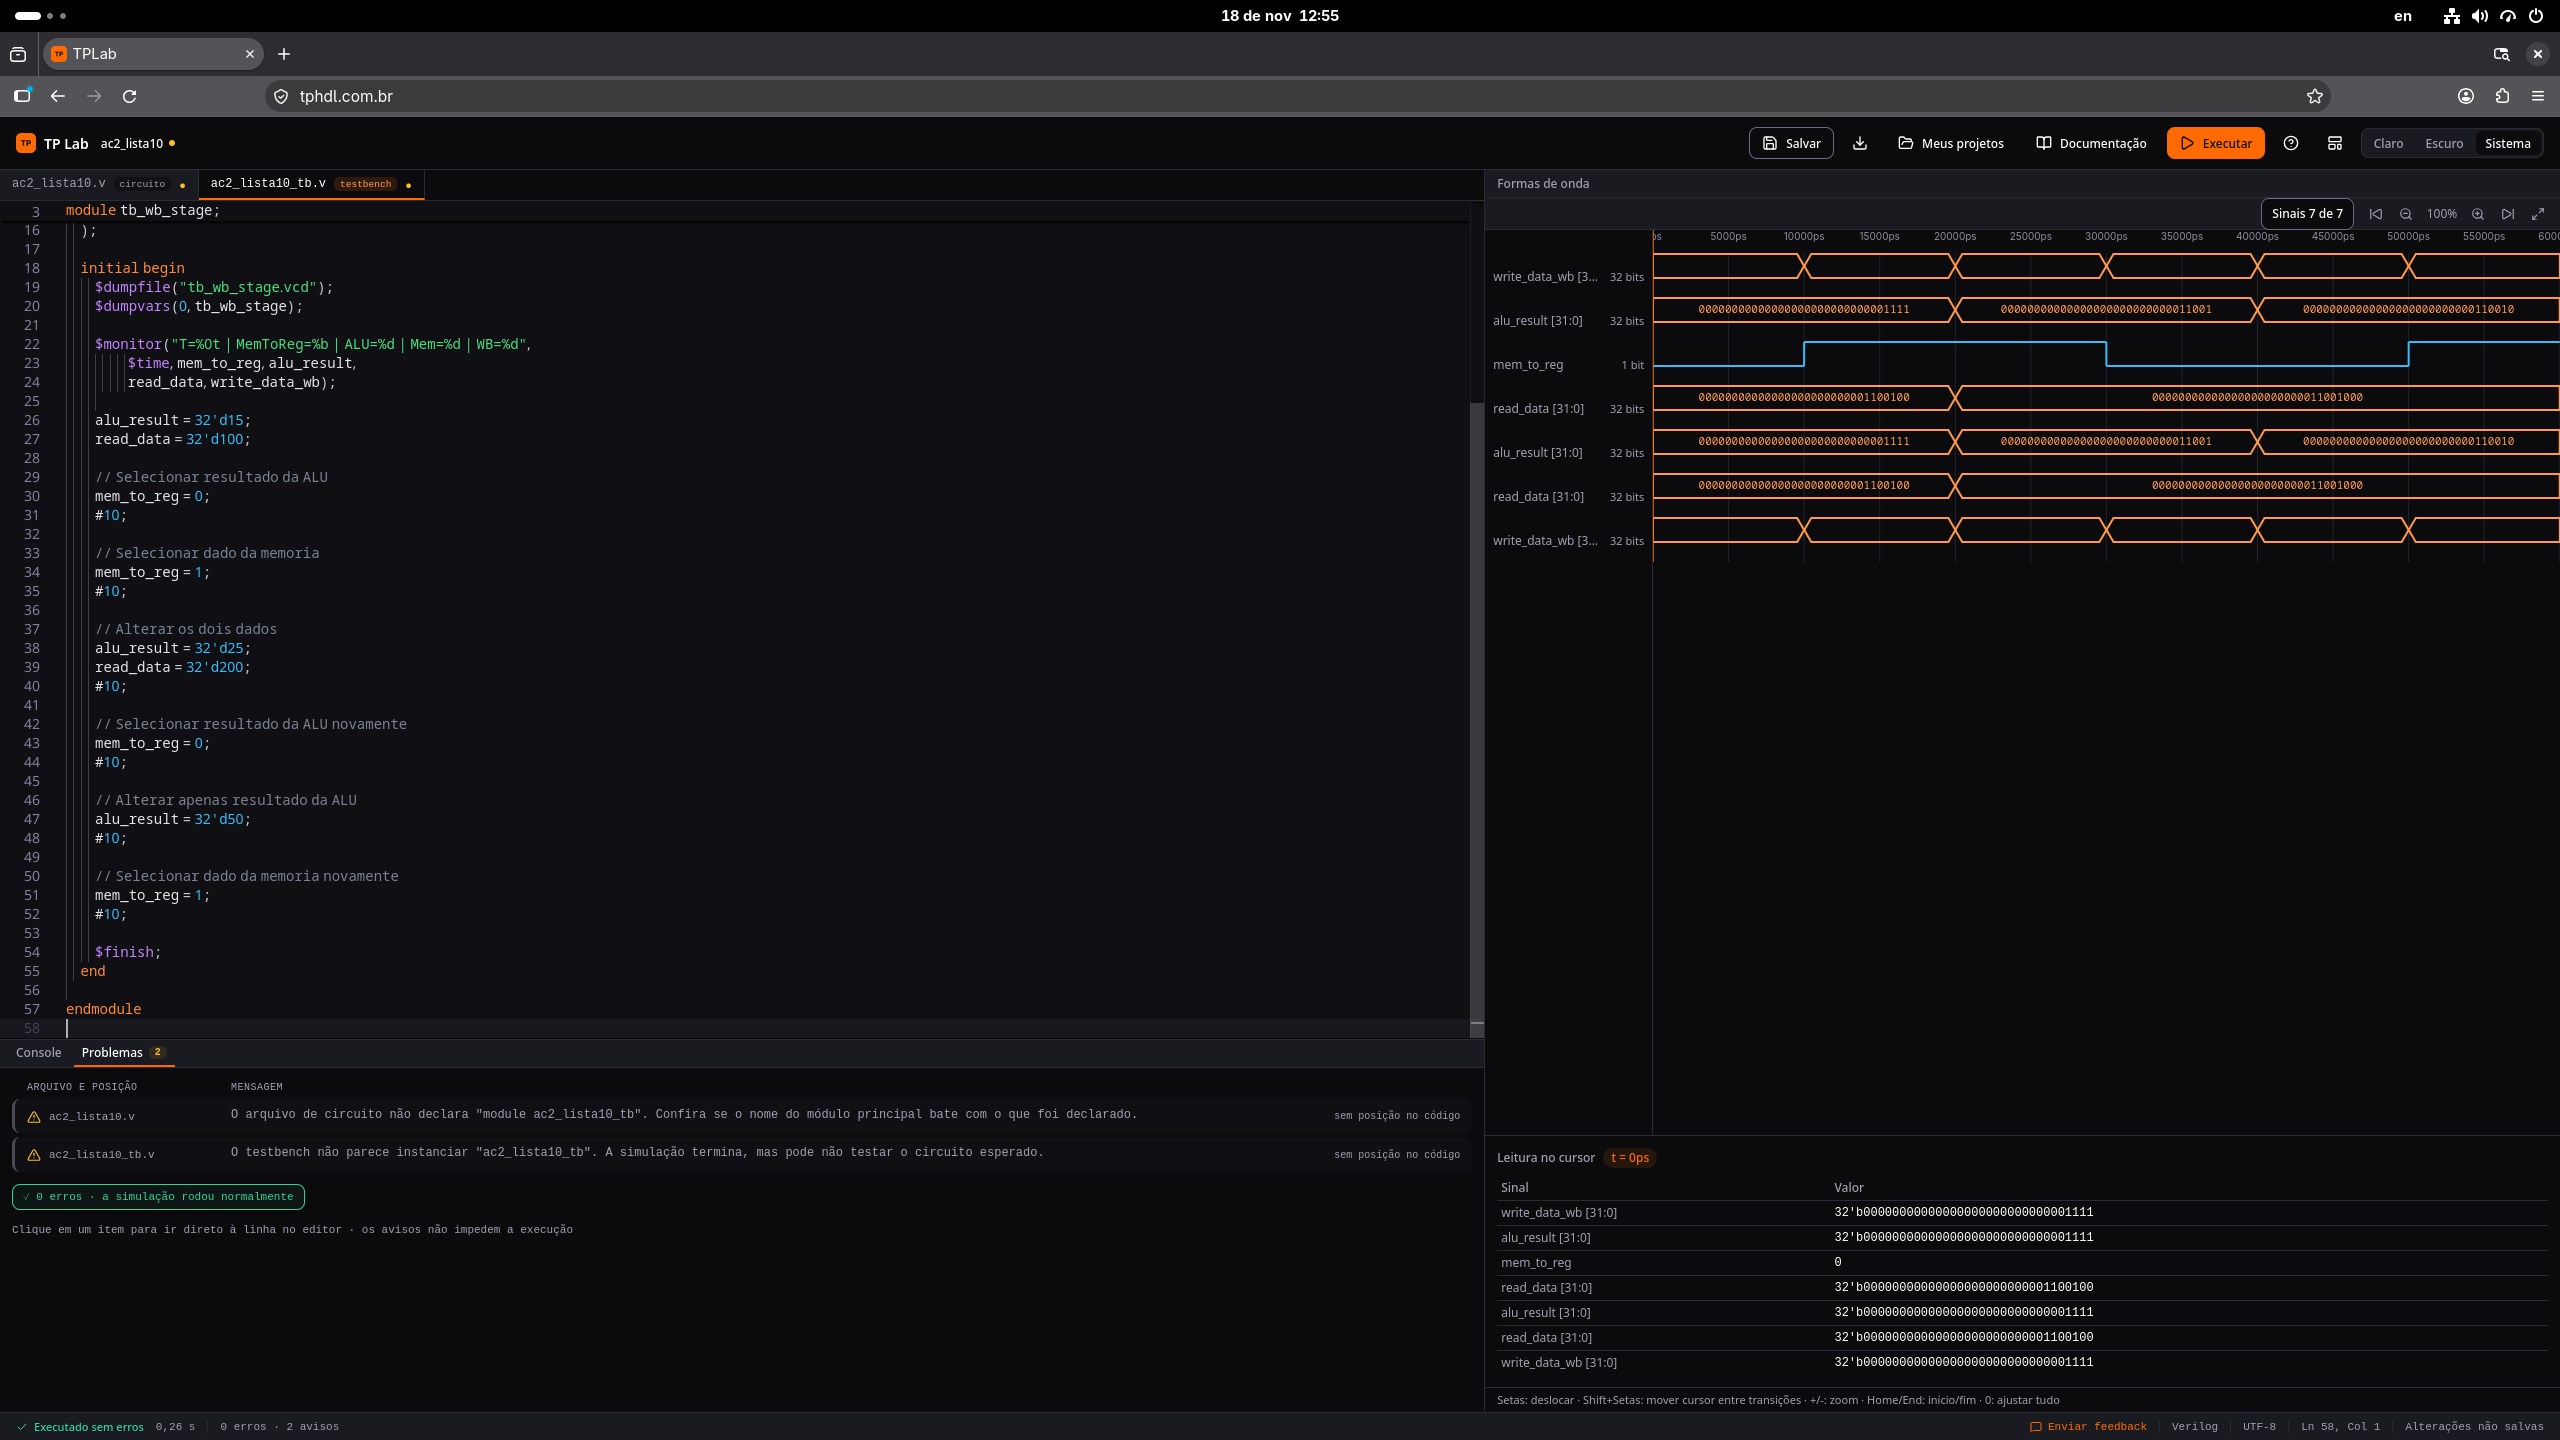
\includegraphics[scale=0.15]{tb_wb_stage}
\end{figure}

\clearpage\subsection{Bloco Top-Level: RISC-V}
\begin{figure}[h]
\centering
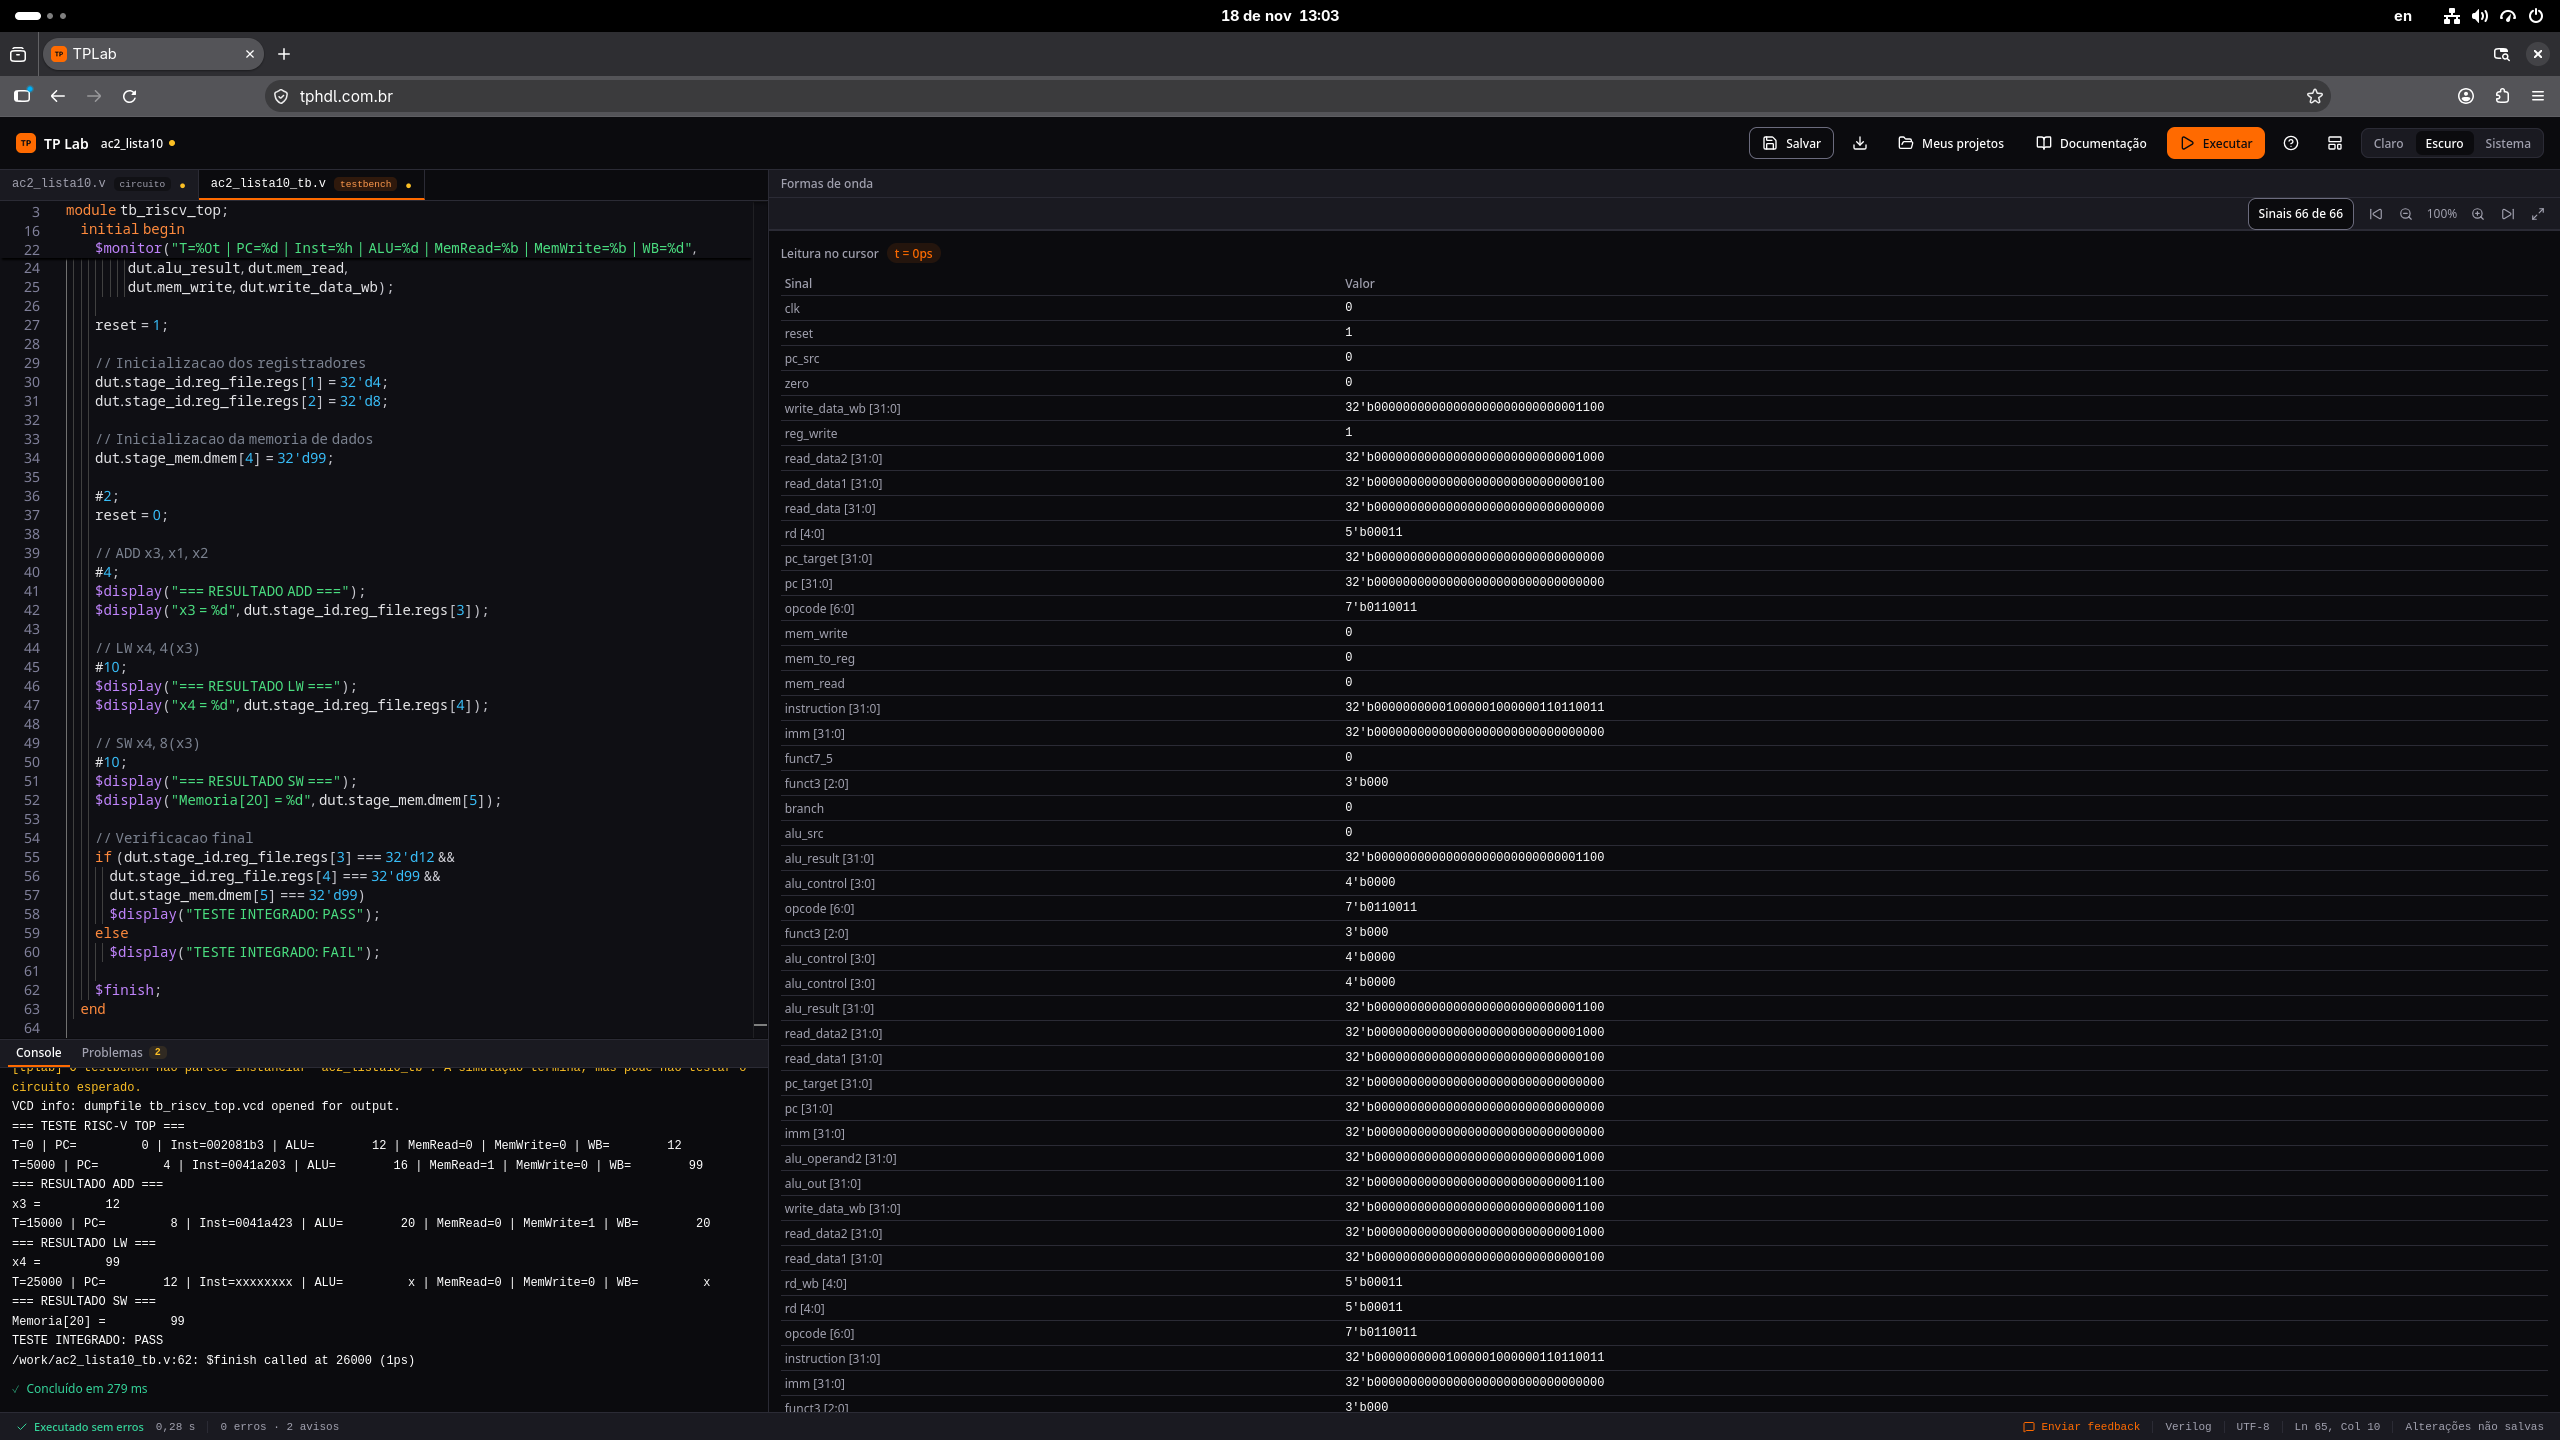
\includegraphics[scale=0.15]{tb_riscv_top}
\end{figure}

\end{document}
